\documentclass[a4paper, 11pt]{article}
\usepackage[a4paper, total={7in, 10in}]{geometry}

%packages
\usepackage{kantlipsum}
\usepackage{pgfplots}
\usepackage{fancyhdr}
\usepackage{lastpage}
\usepackage{mathtools}
\usepackage{tikz}
\usetikzlibrary{arrows,automata,positioning}
\usepackage{enumitem}
\usepackage{amsfonts}
\usepackage{scalerel}
\usepackage{amssymb}
\usepackage{wasysym}
\usepackage{amsmath}
\usepackage{listings}
\usepackage{algorithm}
\usepackage{algpseudocode}
\usepackage{turnstile}

% Tables
\usepackage{tabularx, multirow}
\usepackage{makecell}
\usepackage{booktabs}
\usepackage{placeins}
% \renewcommand*{\arraystretch}{2}

% Make enumerations more compact
\usepackage{enumitem}
\setitemize{itemsep=0.5pt}
\setenumerate{itemsep=0.75pt}

% for centered slash through \implies and \iff
\usepackage{centernot}

%Checkboxes for multiple choice
\newlist{Checkboxes}{itemize}{2}
\setlist[Checkboxes]{label=$\square$}
\usepackage{pifont}
\newcommand{\cmark}{\ding{51}}%
\newcommand{\correct}{\rlap{$\square$}{\raisebox{2pt}{\hspace{1pt}\cmark}}\hspace{-2.5pt}}



%------------------------------------------------------
%Custom Commands
\def\Z{\mathbb{Z}}
\def\R{\mathbb{R}}
\def\N{\mathbb{N}}
\def\C{\mathbb{C}}
\def\L{\mathcal{L}}
\def\O{\mathcal{O}}
\def\Lre{\mathcal{L}_\text{RE}}
\def\Lr{\mathcal{L}_\text{R}}


% define nice looking boxes
\usepackage[many]{tcolorbox}

% a base set, that is then customised
\tcbset {
  base/.style={
    boxrule=0mm,
    boxsep = 1mm,
    leftrule=1mm,
    left=0.8mm,
    arc=2mm, 
    fonttitle=\bfseries, 
    colbacktitle=black!10!white, 
    coltitle=black, 
    toptitle=0.0mm, 
    bottomtitle=0.0mm,
    title={#1}
  }
}

\definecolor{darkred}{rgb}{0.54, 0, 0}
\newtcolorbox{mainbox}[1]{
  colframe=darkred, 
  base={#1}
}

\newtcolorbox{subbox}[1]{
  colframe=black!20!white,
  base={#1}
}



%-----------------------------------------------------

\DeclareMathOperator*{\Bigcdot}{\scalerel*{\cdot}{\bigodot}}

\setlength{\parindent}{0mm}
\setlength{\parskip}{2mm}

\pgfplotsset{samples=100}
\pgfplotsset{compat=1.18}


\newcommand\myTitle[1]{{\large \textbf {#1}}}
\newcommand\ruleSmall{\vspace{-2mm}\begin{center}\rule{0.4\linewidth}{0.3pt}\end{center}\vspace{-2mm}}
\newcommand\ruleMedium{\begin{center}\rule{0.8\linewidth}{1pt}\end{center}}


%--------------------------------------------------
% HEAD
\pagestyle{fancy}
\fancyhf{}
\setlength{\headheight}{27.5pt}
\rhead{Nicolas Wehrli}
\lhead{ETH Zürich, Autumn 2023}
% page numbering
\cfoot{\thepage}
%--------------------------------------------------

\begin{document}
    %--------------------------------------------------
    % Caption
   \begin{titlepage}
    \begin{center}
        \vspace*{5cm}
        \LARGE \textbf{Theoretische Informatik} \\ Beweise 101
    
        \small\textit{Nicolas Wehrli, ETH Zurich}

        \vspace*{5cm}
        \today
    \end{center}
   
   \end{titlepage}
    %--------------------------------------------------
    %--------------------------------------------------
    %--------------------------------------------------
   \tableofcontents
    \newpage



    \section{Grundbegriffe} % Sections are added in order to organize your presentation into discrete blocks, all sections and subsections are automatically output to the table of contents as an overview of the talk but NOT output in the presentation as separate slides

%------------------------------------------------

	Für eine Menge $A$ bezeichnet $|A|$ die Kardinalität von $A$ und $\mathcal{P}(A) = \{S \mid S \subseteq A\}$ die Potenzmenge von $A$.
		
	 In diesem Kurs definieren wir $\N = \{0,1,2, \dots\}$.


\subsection{Alphabet}


		
	 \begin{mainbox}{Definition Alphabet}
		Eine endliche, nichtleere Menge $\Sigma$ heisst \textbf{Alphabet}. Die Elemente eines Alphabets werden \textbf{Buchstaben (Zeichen, Symbole)} genannt.
	 \end{mainbox}
	 
	 \myTitle{Beispiele}
	 \begin{itemize}
		\item $\Sigma_{\text{bool}} = \{0,1\}$
		\item $\Sigma_{\text{lat}} = \{a, ..., z\}$
		\item $\Sigma_{\text{Tastatur}} = \Sigma_{\text{lat}} \cup \{A, ..., Z, \text{\textvisiblespace}, >, <, (,),...,! \}$
		\item $\Sigma_{\text{logic}} = \{0,1,(,),\land, \lor, \lnot\}$
		\item $\Sigma_{abc} = \{a,b,c\}$ (\textbf{unser Beispiel für weitere Definitionen})
	 \end{itemize}


%------------------------------------------------

\subsection{Wort}


	
	\begin{mainbox}{Definition Wort}
		\begin{itemize}[label = -]
			\item Sei $\Sigma$ ein Alphabet. Ein \textbf{Wort} über $\Sigma$ ist eine endliche (eventuell leere) Folge von Buchstaben aus $\Sigma$.
			\item Das \textbf{leere Wort $\lambda$} ist die leere Buchstabenfolge.
			
			\item Die \textbf{Länge $|w|$} eines Wortes $w$ ist die Länge des Wortes als Folge, i.e. die Anzahl der Vorkommen von Buchstaben in $w$. 
			\item $\Sigma^*$ ist die Menge aller Wörter über $\Sigma$. $\Sigma^+ := \Sigma^* \setminus \{\lambda\}$ ist Menge aller nichtleeren Wörter über $\Sigma$.
			
			\item Seien $x \in \Sigma^*$ und $a \in \Sigma$. Dann ist $|x|_a$ definiert als die Anzahl der Vorkommen von $a$ in $x$.
		\end{itemize}
	 \end{mainbox}
	 Achtung Metavariablen! I.e. Das $a$ in der Definition ist steht für einen beliebigen Buchstaben aus $\Sigma$ und \textbf{nicht} nur für den Buchstaben '$a$', der in $\Sigma$ sein könnte.  



	\myTitle{Bemerkungen}
	
	\begin{itemize}[label = -]
		
		\item Wir schreiben Wörter ohne Komma, i.e. eine Folge $x_1,x_2,...,x_n$ schreiben wir $x_1x_2...x_n$.
		\item $|\lambda| = 0$ aber $|\text{\textvisiblespace}| = 1$ von $\Sigma_{\text{Tastatur}}$.
		\item Der Begriff \textbf{Wort} als Fachbegriff der Informatik entspricht \textbf{nicht} der Bedeutung des Begriffs Wort in natürlichen Sprachen!
		\item E.g. Mit \textvisiblespace \ kann der Inhalt eines Buches oder ein Programm als ein Wort über $\Sigma_{\text{Tastatur}}$ betrachtet werden.
	 \end{itemize}
	 
	 \myTitle{Beispiel}
	 Verschiedene Wörter über $\Sigma_{abc}$:

	 $a$, $aa$, $aba$, $cba$, $caaaab$ etc.



	
	\begin{mainbox}{}
		Die \textbf{Verkettung (Konkatenation)} für ein Alphabet $\Sigma$ ist eine Abbildung Kon$: \Sigma^* \times \Sigma^* \to \Sigma^*$, so dass 
		$$\text{Kon}(x, y) = x \cdot y = xy$$
		für alle $x, y \in \Sigma^*$.
	\end{mainbox}
	
	\begin{itemize}[label=-]
		\item Die Verkettung Kon (i.e. Kon von einem Kon (über das gleiche Alphabet $\Sigma$)) ist eine assoziative Operation über $\Sigma^*$.
		$$\text{Kon}(u, \text{Kon}(v, w)) = \text{Kon}(\text{Kon}(u, v), w), \ \forall u,v,w \in \Sigma^*$$
		\item $x\cdot \lambda = \lambda \cdot x = x, \ \forall x \in \Sigma^*$
		\item $\implies$ ($\Sigma^*$, Kon) ist ein Monoid mit neutralem Element $\lambda$.
		\item Kon nur kommutativ, falls $|\Sigma| = 1$.
		\item $|xy|=|x\cdot y| = |x|+|y|$. (Wir schreiben ab jetzt $xy$ statt Kon($x$, $y$))
	\end{itemize}



	\myTitle{Beispiel}

	Wir betrachten wieder $\Sigma_{abc}$. Sei $x = abba$, $y = cbcbc$, $z = aaac$.
	\begin{itemize}[label=-]
		\item Kon($x, \text{Kon}(y, z)) = $  $\text{Kon}(x, yz) = xyz = abbacbcbcaaac$
		\item $|xy| =$$ |abbacbcbc| = 9 = 4 + 5 = |abba| + |cbcbc| = |x| + |y|$
	\end{itemize}
	

	



	
	\begin{mainbox}{}
		Für eine Wort $a = a_1a_2...a_n$, wobei $\forall i \in \{1,2, ..., n\}. \ a_i \in \Sigma$, 
		bezeichnet $a^\text{R} = a_na_{n-1}...a_1$ die \textbf{Umkehrung (Reversal)} von $a$.
	\end{mainbox}
	
	\begin{mainbox}{}
		Sei $\Sigma$ ein Alphabet. Für alle $x \in \Sigma^*$ und alle $i \in \N$ definieren wir die $i$-te \textbf{Iteration} $x^i$ von $x$ als 
		$$x^0 = \lambda, x^1 = x \text{ und } x^i = xx^{i-1}.$$
	\end{mainbox}



	\myTitle{Beispiel}

	Wir betrachten wieder $\Sigma_{abc}$. Sei $x = abba$, $y = cbcbc$, $z = aaac$.
	\begin{itemize}[label = -]
		\item $z^\text{R} =$  $ (aaac)^\text{R} = caaa$
		\item $x^\text{R} =$  $ (abba)^\text{R} = abba$
		\item $x^0 = $  $ \lambda$
		\item  $y^2 = $ $yy^{2-1}= yy = cbcbccbcbc$
		\item $z^3 =$  $zz^2= zzz = aaacaaacaaac$
		\item $(x^\text{R}z^\text{R})^\text{R} = $ $((abba)^\text{R}(aaac)^\text{R})^\text{R} = (abbacaaa)^\text{R} = aaacabba$
	\end{itemize}

	



	
	\begin{mainbox}{}
		Seien $v, w \in \Sigma^*$ für ein Alphabet $\Sigma$.
		\begin{itemize}[label=-]
			\item $v$ heisst ein \textbf{Teilwort} von $w$ $\iff$ $\exists x,y \in \Sigma^*: \ w = xvy$
			\item $v$ heisst ein \textbf{Präfix} von $w$ $\iff$ $\exists y \in \Sigma^*: \ w = vy$
			\item $v$ heisst ein \textbf{Suffix} von $w$ $\iff$ $\exists x \in \Sigma^*: \ w = xv$
			\item $v \neq \lambda$ heisst ein \textbf{echtes} Teilwort (Präfix, Suffix) von $w$ $\iff$ $v \neq w$ und $v$ Teilwort(Präfix, Suffix) von $w$
		\end{itemize}
	\end{mainbox}



	\myTitle{Beispiel}

	Wir betrachten wieder $\Sigma_{abc}$. Sei $x = abba$, $y = cbcbc$, $z = aaac$.
	\begin{itemize}[label=-]
		\item $bc$ ist ein echtes Suffix von $y$
		\item $abba$ ist kein echtes Teilwort von $x$.
		\item $cbcb$ ist ein echtes Teilwort und echtes Präfix von $y$.
		\item $ac$ ist ein echtes Suffix.
		\item $abba$ ist ein Suffix, Präfix und Teilwort von $x$.
	\end{itemize}

    \myTitle{Aufgabe 1}

	Sei $\Sigma$ ein Alphabet und sei $w \in \Sigma^*$ ein Wort der Länge $n \in \N \setminus \{0\}$. Wie viele unterschiedliche Teilwörter kann $w$ höchstens haben?

	\myTitle{Lösung}

	Wir haben $w = w_1w_2...w_n$ mit $w_i \in \Sigma$ für $i = 1, ...,n$. Wie viele Teilwörter beginnen mit $w_1$? Wie viele Teilwörter beginnen mit $w_2$?
	 
	
	Wir haben also $n + (n-1) + ... + 1 = \frac{n(n+1)}{2}$ Teilwörter. Etwas fehlt aber in unserer Berechnung\dots
	
	
	Das leere Wort $\lambda$ ist auch ein Teilwort! Also haben wir $\frac{n(n+1)}{2}+ 1$ Teilwörter. 

    \vspace*{1cm}
    \myTitle{Aufgabe 2}

	Sei $\Sigma = \{a, b, c\}$ und $n \in \N$. Bestimme die Anzahl der Wörter aus $\Sigma^n$, die das Teilwort $a$ enthalten.
	
    \myTitle{Lösung}
    
	In solchen Aufgaben ist es manchmal einfach, das Gegenteil zu berechnen und so auf die Lösung zu kommen. Wie viele Wörter aus $\Sigma^n$ enthalten das Teilwort $a$ \textbf{nicht}?

	
	Da wir jetzt die Anzahl Wörter der Länge $n$ wollen, die nur $b$ und $c$ enthalten, kommen wir auf $|\{b,c\}|^n = 2^n$.
	
	Daraus folgt, dass genau $|\Sigma|^n - 2^n = 3^n -2^n$ Wörter das Teilwort $a$ enthalten.
    \vspace*{1cm}

    \myTitle{Aufgabe 3}

	Sei $\Sigma= \{a,b,c\}$ und $n \in \N \setminus\{0\}$. Bestimme die Anzahl der Wörter aus $\Sigma^n$, die das Teilwort $aa$ nicht enthalten.

	\myTitle{Lösung}

	Wir bezeichnen die Menge aller Wörter mit Länge $n$ über $\Sigma$, die $aa$ nicht enthalten als $L_n$.

	Schauen wir mal die ersten zwei Fälle an:
	\begin{itemize}
		\item $L_1 = \{a,b,c\} \implies |L_1| = 3$
		\item $L_2 = \{ab, ac, ba, bb, bc, ca, cb, cc\} \implies |L_2| = 8$ 
	\end{itemize}
	
	Nun können wir für $m \geq 3$ jedes Wort $w \in L_m$ als Konkatination $w = x \cdot y \cdot z$ schreiben, wobei wir zwei Fälle unterscheiden:
	
	\begin{enumerate}[label= (\alph*)]
		
		\item $\mathbf{z \neq a}$
		
		In diesem Fall kann $y \in \{a,b,c\}$ sein, ohne dass die Teilfolge $aa$ entsteht und somit ist $xy$ ein beliebiges Wort aus $L_{m-1}$. 
		
		Dann könnten wir alle Wörter in diesem Case durch $L_{m-1}\cdot \{b,c\}$ beschreiben, was uns die Kardinalität $2 \cdot |L_{m-1}|$ gibt.
		
		\item $\mathbf{z = a}$
		
		In diesem Fall muss $y \neq a$ sein, da sonst $aa$ entstehen würde. 
		
		Somit kann $xy$ nur in $b$ oder $c$ enden. $x$ kann aber ein beliebiges Wort der Länge $m-2$ sein. 
		
		Deshalb können wir alle Wörter in diesem Case durch $L_{m-2}\cdot\{b, c\} \cdot \{a\}$ beschreiben. Kardinalität: $2 \cdot |L_{m-2}|$.
	\end{enumerate}

    Daraus folgt $$|L_n| = \begin{cases}
        3 &  n = 1\\
        8 & n = 2\\
        2|L_{n-1}|+ 2|L_{n-2}| &n \geq 3
    \end{cases}$$

\vspace*{1cm}

	
	\begin{mainbox}{}
		Sei $\Sigma = \{s_1,s_2, ...,s_m\}, m \geq 1$, ein Alphabet und sei $s_1 < s_2 < ... <s_m$ eine Ordnung auf $\Sigma$. Wir definieren die \textbf{kanonische Ordnung} auf $\Sigma^*$ für $u, v \in \Sigma^*$ wie folgt:
		\begin{align*}
			u < v \iff &|u| < |v| \lor (|u| = |v| \land u = x\cdot s_i \cdot u' \land x \cdot s_j \cdot v') \\
			&\text{ für irgendwelche } x, u', v' \in \Sigma^* \text{ und } i < j. 
		\end{align*}
	\end{mainbox}



	Sei $\Sigma_{abc} = \{a, b, c\}$ und wir betrachten folgende Ordnung auf $\Sigma_{abc}$: $c < a < b$.

	Was wäre die kanonische Ordnung folgender Wörter?

	$c$, $abc$, $aaac$, $aaab$, $bacc$, $a$, $\lambda$

	
	$\lambda$, $c$, $a$, $abc$, $aaac$, $aaab$, $bacc$


%------------------------------------------------

\subsection{Sprache}


	
	\begin{mainbox}{}
	 Eine \textbf{Sprache $L$} über einem Alphabet $\Sigma$ ist eine Teilmenge von $\Sigma^*$. 
	\end{mainbox}
	\begin{itemize}[label=-]
		\item Das Komplement \textbf{$L^\complement$} der Sprache $L$ bezüglich $\Sigma$ ist die Sprache $\Sigma^* \setminus L$.
		\item $L_\emptyset = \emptyset$ ist die \textbf{leere Sprache}.
		\item $L_\lambda = \{\lambda\}$ ist die einelementige Sprache, die nur aus dem leeren Wort besteht.
	\end{itemize}
	
	\myTitle{Konkatenation von Sprachen}
	\begin{mainbox}{}
		Sind $L_1$ und $L_2$ Sprachen über $\Sigma$, so ist 
		$$L_1 \cdot L_2 = L_1L_2 = \{vw \mid v \in L_1 \text{ und } w \in L_2\}$$
		die \textbf{Konkatenation} von $L_1$ und $L_2$. 
	\end{mainbox}



	\begin{mainbox}{}
		Ist $L$ eine Sprache über $\Sigma$, so definieren wir
		\begin{align*}
			&L^0 := L_{\lambda} \text{ und } L^{i+1} := L^{i}\cdot L \text{ für alle } i \in \N,\\
			&L^* = \bigcup_{i \in \N}L^i \text{ und } L^+ = \bigcup_{i \in \N \setminus \{0\}} L^i = L \cdot L^*.
		\end{align*}
		$L^*$ nennt man den \textbf{Kleene'schen Stern} von $L$.
	\end{mainbox}
	Man bemerke, dass $\Sigma^i = \{x \in \Sigma^* \mid |x| = i\}$, $L_\emptyset L = L_\emptyset = \emptyset$ und $L_\lambda \cdot L = L$.
	



	Mögliche Sprachen über $\Sigma_{abc}$
	\begin{itemize}[label=-]
		\item $L_1 = \emptyset$
		\item $L_2 = \{\lambda\}$
		\item $L_3 = \{\lambda, ab, baca\}$
		\item $L_4 = \Sigma_{abc}^*$, $L_5 = \Sigma_{abc}^+$, $L_6 = \Sigma_{abc}$ oder $L_7 = \Sigma_{abc}^{27}$
		\item $L_8 = \{c\}^* = \{c^i \mid i \in \N\}$
		\item $L_9 = \{a^p \mid p \text{ ist prim.}\}$
		\item $L_{10} = \{c^{i}a^{3i^2}ba^ic \mid i \in \N\}$
	\end{itemize}
	$\lambda$ ist ein Wort über jedes Alphabet. Aber es muss nicht in jeder Sprache enthalten sein!


% --------------------------------------------------------------------------------------


	\begin{subbox}{}
		Seien $L_1$, $L_2$ und $L_3$ Sprachen über einem Alphabet $\Sigma$. Dann gilt
		\begin{align}
			&L_1L_2 \cup L_1L_3 = L_1(L_2 \cup L_3) \\
			&L_1(L_2 \cap L_3) \subseteq L_1L_2 \cap L_1L_3
		\end{align}
	\end{subbox}
	Weshalb nicht '$=$' bei $(2)$?

	Sei $\Sigma = \Sigma_{\text{bool}} = \{0,1\}$, $L_1 = \{\lambda, 1\}$, $L_2 = \{0\}$ und $L_3 = \{10\}$.

	Dann haben wir $L_1(L_2 \cap L_3) = \emptyset \neq \{10\} = L_1L_2 \cap L_1L_3$.

	\textit{Beweise im Buch/Vorlesung}



	\begin{mainbox}{Homomorphismus}
		Seien $\Sigma_1$ und $\Sigma_2$ zwei beliebige Alphabete. Ein Homomorphismus von $\Sigma_1^*$ nach $\Sigma_2^*$ ist jede Funktion $h: \Sigma_1^* \to \Sigma_2^*$ mit den folgenden Eigenschaften:
		\begin{enumerate}[label=(\roman*)]
			\item $h(\lambda) = \lambda$ und 
			\item $h(uv) = h(u)\cdot h(v)$ für alle $u, v \in \Sigma_1^*$.
		\end{enumerate}
	\end{mainbox}
	Wir können Probleme etc. in anderen Alphabeten kodieren. So wie wir verschiedenste Konzepte, die wir auf Computer übertragen in $\Sigma_{\text{bool}}$ kodieren.


\section{Algorithmische Probleme}

	Mathematische Definition folgt in Kapitel 4 (Turingmaschinen).
	\begin{mainbox}{Algorithmen - Provisorische Definition}
		Vorerst betrachten wir Programme, die \textbf{für jede zulässige Eingabe halten und eine Ausgabe liefern}, als Algorithmen.

		Wir betrachten ein Programm (Algorithmus) $A$ als Abbildung $A: \Sigma_1^* \to \Sigma_2^*$ für beliebige Alphabete $\Sigma_1$ und $\Sigma_2$. Dies bedeutet, dass 
		\begin{enumerate}[label=(\roman*)]
			\item die Eingaben als Wörter über $\Sigma_1$ kodiert sind,
			\item die Ausgaben als Wörter über $\Sigma_2$ kodiert sind und
			\item $A$ für jede Eingabe eine eindeutige Ausgabe bestimmt.
		\end{enumerate}
	\end{mainbox}

	$A$ und $B$ äquivalent $\iff$ Eingabealphabet $\Sigma$ gleich, $A(x) = B(x), \forall x \in \Sigma^*$
	
	Ie. diese Notion von ''Äquivalenz'' bezieht sich nur auf die Ein und Ausgabe.




	\begin{mainbox}{Entscheidungsproblem}
		Das \textbf{Entscheidungsproblem $(\Sigma, L)$} für ein gegebenes Alphabet $\Sigma$ und eine gegebene Sprache $L \subseteq \Sigma^*$ ist, für jedes $x \in \Sigma^*$ zu entscheiden, ob 
		$$x \in L \text{ oder } x \notin L.$$
		Ein Algorithmus $A$ \textbf{löst} das Entscheidungsproblem $(\Sigma, L)$, falls für alle $x \in \Sigma^*$ gilt:
		$$A(x) = \begin{cases}
			1, &\text{falls }x \in L,\\
			0, &\text{falls }x \notin L.
		\end{cases}$$
		Wir sagen auch, dass $A$ die Sprache $L$ erkennt.
	\end{mainbox}






	\begin{subbox}{Rekursive Sprachen}
		Wenn für eine Sprache $L$ ein Algorithmus existiert, der $L$ erkennt, sagen wir, dass $L$ \textbf{rekursiv} ist.
	\end{subbox}

	Wir sind oft an spezifischen Eigenschaften von Wörtern aus $\Sigma^*$ interessiert, die wir mit einer Sprache $L \subseteq \Sigma^*$ beschreiben können.

	Dabei sind dann $L$ die Wörter, die die Eigenschaft haben und $L^\complement = \Sigma^* \setminus L$ die Wörter, die diese Eigenschaft nicht haben. 

	Jetzt ist die allgemeine Formulierung von Vorteil!



	\begin{enumerate}[label=\roman*.]
		\item \textbf{Primzahlen finden}: 
		
		Entscheidungsproblem $(\Sigma_{\text{bool}}, L_p)$ wobei \\
        $L_p = \{x \in (\Sigma_{\text{bool}})^* \mid \text{Nummer}(x) \text{ ist prim}\}$.
		\item \textbf{Syntaktisch korrekte Programme}: 
		
		Entscheidungsproblem $(\Sigma_{\text{Tastatur}}, L_{C++})$ wobei\\ 
        $L_{C++} = \{x \in (\Sigma_{\text{Tastatur}})^* \mid x \text{ ist ein syntaktisch korrektes C++ Programm}\}$.
		\item \textbf{Hamiltonkreise finden: } 
		
		Entscheidungsproblem $(\Sigma, \text{HK})$ wobei $\Sigma = \{0,1,\#\}$ und \\
        HK$=\{x \in \Sigma^* \mid x \text{ kodiert einen Graphen, der einen Hamiltonkreis enthält.}\}$
	\end{enumerate}
	Äquivalenzprobleme $\subset$ Entscheidungsprobleme



	\begin{mainbox}{}
		Seien $\Sigma$ und $\Gamma$ zwei Alphabete. 
		\begin{itemize}[label=-]
			\item Wir sagen, dass ein Algorithmus $A$ eine \textbf{Funktion (Transformation) $f: \Sigma^* \to \Gamma^*$ berechnet (realisiert)}, falls
			$$A(x) = f(x) \text{ für alle } x \in \Sigma^*$$
			\item Sei $R \subseteq \Sigma^* \times \Gamma^*$ eine Relation in $\Sigma^*$ und $\Gamma^*$. Ein Algorithmus \textbf{$A$ berechnet $R$} 
			(bzw. \textbf{löst das Relationsproblem $R$}), falls für jedes $x \in \Sigma^*$, für das ein $y \in \Gamma^*$ mit $(x,y) \in R$ existiert, gilt:
			$$(x, A(x)) \in R$$
		\end{itemize}
		
	\end{mainbox}




	\begin{mainbox}{Optimierungsproblem}
		Ein \textbf{Optimierungsproblem} ist ein $6$-Tupel $\mathcal{U} = (\Sigma_I, \Sigma_O, L, M, \text{cost}, \text{goal})$, wobei:
		\begin{enumerate}[label=(\roman*)]
			\item $\Sigma_I$ ist ein Alphabet (genannt \textbf{Eingabealphabet}),
			\item $\Sigma_O$ ist ein Alphabet (genannt \textbf{Ausgabealphabet}),
			\item $L \subseteq \Sigma_I^*$ ist die Sprache der \textbf{zulässigen Eingaben} (als Eingaben kommen nur Wörter in Frage, die eine sinnvolle Bedeutung haben). 
			Ein $x \in L$ wird ein \textbf{Problemfall (Instanz) von $\mathcal{U}$} genannt.
			\item $M$ ist eine Funktion von $L$ nach $\mathcal{P}(\Sigma_O^*)$, und für jedes $x \in L$ ist $M(x)$ die \textbf{Menge der zulässigen Lösungen für $x$},
			\item \textbf{cost} ist eine Funktion, \textbf{cost}$: \bigcup_{x \in L}(\mathcal{M}(x)\times\{x\}) \to \R^+$, genannt \textbf{Kostenfunktion},
			\item \textbf{goal} $\in \{\text{Minimum}, \text{Maximum}\}$ ist das \textbf{Optimierungsziel}.
		\end{enumerate}	
        Eine zulässige Lösung $\alpha \in \mathcal{M}(x)$ heisst \textbf{optimal} für den Problemfall $x$ des Optimierungsproblems $\mathcal{U}$, falls 
		\begin{center}
			cost($\alpha, x$) $= \textbf{Opt}_\mathcal{U}(x) = \text{ goal}\{\text{cost}(\beta, x) \mid \beta \mathcal{M}(x)\}$.
		\end{center}
		Ein Algorithmus $A$ \textbf{löst $\mathcal{U}$}, falls für jedes $x \in L$
		\begin{enumerate}[label=(\roman*)]
			\item $A(x) \in \mathcal{M}(x)$
			\item cost$(A(x), x) = \text{ goal}\{\text{cost}(\beta, x) \mid \beta \in \mathcal{M}(x)\}$.
		\end{enumerate} 
	\end{mainbox}

    \section{Kolmogorov Komplexität}
    \subsection{Theorie}
        \begin{mainbox}{Algorithmen generieren Wörter}
            Sei $\Sigma$ ein Alphabet und $x \in \Sigma^*$. Wir sagen, dass ein Algorithmus $A$ das Wort $x$ \textbf{generiert}, falls $A$ für die Eingabe $\lambda$ die Ausgabe $x$ liefert.
        \end{mainbox}
        Beispiel:
        \begin{lstlisting}[mathescape = true, escapeinside={(*}{*)}]
            $A_n$: 	begin
                    for $i$ = 1 to $n$;
                        write(01);
                end
           \end{lstlisting}
           $A_n$ generiert $(01)^n$.
    
        \begin{mainbox}{Aufzählungsalgorithmus}
            Sei $\Sigma$ ein Alphabet und sei $L \subseteq \Sigma^*$. $A$ ist ein \textbf{Aufzählungsalgorithmus für $L$}, 
            falls $A$  für jede Eingabe $n \in \N \setminus \{0\}$ die Wortfolge $x_1, ...,x_n$ ausgibt, wobei $x_1, ...,x_n$ die kanonisch $n$ ersten Wörter in $L$ sind.
        \end{mainbox}
    
        \textbf{Aufgabe 2.21}
        
        Beweisen Sie, dass eine Sprache $L$ genau dann rekursiv ist, wenn ein Aufzählungsalgorithmus für $L$ existiert.
        \begin{mainbox}{}
            Das \textbf{Entscheidungsproblem $(\Sigma, L)$} für ein gegebenes Alphabet $\Sigma$ und eine gegebene Sprache $L \subseteq \Sigma^*$ ist, für jedes $x \in \Sigma^*$ zu entscheiden, ob 
            $$x \in L \text{ oder } x \notin L.$$
            Ein Algorithmus $A$ \textbf{löst} das Entscheidungsproblem $(\Sigma, L)$, falls für alle $x \in \Sigma^*$ gilt:
            $$A(x) = \begin{cases}
                1, &\text{falls }x \in L,\\
                0, &\text{falls }x \notin L.
            \end{cases}$$
            Wir sagen auch, dass $A$ die Sprache $L$ erkennt.
        \end{mainbox}
    
        $L$ rekursiv $(\implies)$ existiert Aufzählungsalgorithmus:
    
        Sei $A$ ein Algorithmus, der $L$ erkennt. Wir beschreiben nun einen Aufzählungsalgorithmus $B$ konstruktiv. 
    
        \begin{algorithm}[H]
            \caption{$B(\Sigma, n)$}
            \begin{algorithmic}
                \State i $\leftarrow$ 0
                \While{i $\leq n$}
                    \State $w$ $\leftarrow$ kanonisch nächstes Wort über $\Sigma^*$
                    \If{$A(w) = 1$}
                    \State print($w$)
                    \State $i \leftarrow i + 1$
                    \EndIf 
                \EndWhile
            \end{algorithmic}
        \end{algorithm}
    
        Aufzählungsalgorithmus $B$ $\implies$ $L$ rekursiv:
    
        \begin{algorithm}[H]
            \caption{$A(\Sigma, w)$}
            \begin{algorithmic}
                \State$n \leftarrow$ $|\Sigma|^{|w| + 1}$
                \State $L \leftarrow B(\Sigma, n)$
                \If{$w \in L$}
                \State print(1)
                \Else
                \State print(0)
                \EndIf
            \end{algorithmic}
        \end{algorithm}
        Es gibt ein kleines Problem. $B$ könnte unendlich lange laufen, falls $n > |L|$.\\ 
        Es sollte nicht so schwierig sein, $B$ zu modifizieren, dass es die Berechnung aufhört, falls es keine weiteren Wörter in $L$ gibt.
    
    
    
        \myTitle{Information messen}

        Wir beschränken uns auf $\Sigma_{\text{bool}}$
        \begin{mainbox}{Kolmogorov-Komplexität}
            Für jedes Wort $x \in (\Sigma_{\text{bool}})^*$ ist die \textbf{Kolmogorov-Komplexität $K(x)$ des Wortes $x$} das Minimum der binären Längen, der Pascal-Programme, die $x$ generieren.
        \end{mainbox}
        $K(x)$ ist die kürzestmögliche Länge einer Beschreibung von $x$.
    
        Die einfachste (und triviale) Beschreibung von $x$, ist wenn man $x$ direkt angibt.
    
        $x$ kann aber eine Struktur oder Regelmässigkeit haben, die eine Komprimierung erlaubt.
    
        Welche Programmiersprache gewählt wird verändert die Kolmogorov-Komplexität nur um eine Konstante. (Satz 2.1)
    
    
    
        \textbf{Beispiel}
        
        Sei $w = 0101010101010101010101010101010101010101$. Die Länge von $w$ ist $|w| = 40$ und die triviale Beschreibunglänge wäre wie gegeben $40$.
    
        Aber durch die Regelmässigkeit von einer $20$-fachen Wiederholung der Sequenz $01$, können $w$ auch durch $(01)^{20}$ beschreiben. 
        Hierbei ist die Beschreibungslänge ein wenig mehr als $4$ Zeichen.
    
    
    
        \textbf{Grundlegende Resultate}
        \begin{mainbox}{}
            Es existiert eine Konstante $d$, so dass für jedes $x \in (\Sigma_{\text{bool}})^*$
            $$K(x) \leq |x| + d$$
        \end{mainbox}
    
        \begin{mainbox}{}
            Die \textbf{Kolmogorov-Komplexität einer natürlichen Zahl $n$} ist $K(n) = K(\text{Bin}(n))$.
        \end{mainbox}
    
        
        \begin{mainbox}{Lemma 2.5 - Nichtkomprimierbar}
            Für jede Zahl $n \in \N \setminus\{0\}$ existiert ein Wort $w_n \in (\Sigma_{\text{bool}})^n$, so dass 
            $$K(w_n) \geq |w_n| = n$$
        \end{mainbox}
        \textbf{Beweis}

        Es gibt $2^n$ Wörter $x_1, ..., x_{2^n}$ über $\Sigma_{bool}$ der Länge $n$. 
        Wir bezeichnen $C(x_i)$ als den Bitstring des kürzesten Programms, der $x_i$ generieren kann. Es ist klar, dass für $i \neq j: C(x_i) \neq C(x_j)$.
    
        Die Anzahl der nichtleeren Bitstrings, i.e. der Wörter der Länge $< n$ über $\Sigma_{bool}$ ist:
        $$\sum_{i = 1}^{n-1} 2^i = 2^n - 2 < 2^n$$
        Also muss es unter den Wörtern $x_1, ...,x_{2^n}$ mindestens ein Wort $x_k$ mit $K(x_k) \geq n$ geben.
        
        \hspace*{0pt}\hfill$\blacksquare$
    
    
    
        \textbf{Satz 2.1 - Programmiersprachen}

        Für jedes Wort $x \in (\Sigma_{\text{bool}})^*$ und jede Programmiersprache $A$ sei $K_A(x)$ die Kolmogorov-Komplexität von $x$ bezüglich der Programmiersprache $A$.
        \begin{mainbox}{}
            Seien $A$ und $B$ Programmiersprachen. Es existiert eine Konstante $c_{A,B}$, die nur von $A$ und $B$ abhängt, so dass 
            $$|K_A(x) -K_B(x)|\leq c_{A,B}$$
            für alle $x \in (\Sigma_{\text{bool}})^*$.
        \end{mainbox}
        \textit{Beweis im Buch/Vorlesung}
    
        \begin{mainbox}{Ein zufälliges Wort}
            Ein Wort $x \in (\Sigma_{\text{bool}})^*$ heisst \textbf{zufällig}, falls $K(x) \geq |x|$. 
            
            Eine Zahl $n$ heisst \textbf{zufällig}, falls $K(n) = K(\text{Bin}(n)) \geq \left\lceil\log_2(n + 1) \right\rceil - 1$.
        \end{mainbox}
        Jede Binär-Darstellung beginnt immer mit einer $1$, deshalb können wir die Länge der Binär-Darstellung um $1$ verkürzen.
    
        Zufälligkeit hier bedeutet, dass ein Wort völlig unstrukturiert ist und sich nicht komprimieren lässt. Es hat nichts mit Wahrscheinlichkeit zu tun.
    
        \begin{mainbox}{Satz 2.2}
            Sei $L$ eine Sprache über $\Sigma_{\text{bool}}$. Sei für jedes $n \in \N \setminus \{0\}$, $z_n$ das $n$-te Wort in $L$ bezüglich der kanonischen Ordnung. 
            Wenn ein Programm $A_L$ existiert, das das Entscheidungsproblem $(\Sigma_{\text{bool}}, L)$ löst, dann gilt für alle $n \in \N\setminus\{0\}$, dass
            $$K(z_n) \leq \left\lceil\log_2(n+1)\right\rceil + c$$
            wobei $c$ eine von $n$ unabhängige Konstante ist.
        \end{mainbox}
        \textbf{Beweisidee}

        Wir können aus $A_L$, ein Programm entwerfen, dass das kanonisch $n$-te Wort generiert, indem wir in der kanonischen Reihenfolge alle Wörter $x \in (\Sigma_{bool})^*$ durchgehen und mit $A_L$ entscheiden, ob $x \in L$. Dann können wir einen Counter $c$ haben und den Prozess abbrechen, wenn der Counter $c = n$ wird und dann dieses Wort ausgeben.
    
        Wir sehen, dass dieses Programm ausser der Eingabe $n$ immer gleich ist. Sei die Länge dieses Programms $c$, dann können wir für das $n$-te Wort der Sprache $L, z_n,$ die Kolmogorov-Komplexität auf $n$ reduzieren, bzw:
        $$K(z_n) \leq \lceil \log_2(n+1)\rceil + c$$
        \hspace*{0pt}\hfill$\blacksquare$
    
    
    
        \textbf{Primzahlsatz}

        Für jede positive ganz Zahl $n$ sei Prim($n$) die Anzahl der Primzahlen kleiner gleich $n$. 
        \begin{mainbox}{}
            $$\lim_{n \to \infty}\frac{\text{Prim}(n)}{n/\ln n} = 1$$
        \end{mainbox}
        Nützliche Ungleichung
        $$\ln n - \frac{3}{2} < \frac{n}{\text{Prim(n)}} < \ln n - \frac{1}{2}$$
        für alle $n \geq 67$.
    
        \begin{mainbox}{Lemma 2.6 - schwache Version des Primzahlsatzes}
            Sei $n_1, n_2, n_3, ...$ eine steigende unendliche Folge natürlicher Zahlen mit $K(n_i) \geq \lceil \log_2 n_i \rceil / 2$. Für jedes $i \in \N \setminus \{0\}$ sei $q_i$ die grösste Primzahl, die die Zahl $n_i$ teilt. Dann ist die Menge $Q = \{q_i \mid i \in \N \setminus\{0\}\}$ unendlich.
        \end{mainbox}
        \textbf{Beweis: }
        Wir beweisen diese Aussage per Widerspruch:
    
        Nehmen wir zum Widerspruch an, dass die Menge $Q = \{q_i \mid i \in \N \setminus \{0\}\}$ sei endlich. 
        
        Sei $q_m$ die grösste Primzahl in $Q$. Dann können wir jede Zahl $n_i$ eindeutig als 
        $$n_i = q_1^{r_{i, 1}} \cdot q_2^{r_{i,2}} \cdot \cdots \cdot q_m^{r_{i,m}}$$
        für irgendwelche $r_{i,1}, r_{i,2}, ..., r_{i,m} \in \N$ darstellen. Sei $c$ die binäre Länge eines Programms, dass diese $r_{i,j}$ als Eingaben nimmt und $n_i$ erzeugt (A ist für alle $i\in \N$ bis auf die Eingaben $r_{i,1}, ..., r_{i,m}$ gleich).
        
        Dann gilt:
        $$K(n_i) \leq c + 8 \cdot (\lceil \log_2(r_{i,1}+1)\rceil + \lceil \log_2(r_{i,2}+1)\rceil + ... + \lceil \log_2(r_{i,m}+1)\rceil)$$
        Die multiplikative Konstante $8$ kommt daher, dass wir für die Zahlen $r_{i,1}, r_{i,2}, ..., r_{i,m}$ dieselbe Kodierung, wie für den Rest des Programmes verwenden (z.B. ASCII-Kodierung), damit ihre Darstellungen eindeutig voneinander getrennt werden können. Weil  $r_{i,j} \leq \log_2 n_i, \forall j \in \{1, ..., m\}$ erhalten wir 
        $$K(n_i) \leq c + 8m \cdot \lceil \log_2(\log_2 n_i + 1)\rceil, \forall i \in \N \setminus \{0\}$$
       
        Weil $m$ und $c$ Konstanten unabhängig von $i$ sind, kann 
        $$\lceil \log_2 n_i \rceil / 2 \leq K(n_i) \leq c + 8m \cdot \lceil \log_2(\log_2 n_i + 1)\rceil$$
        $$\lceil \log_2 n_i \rceil/2 \leq c + 8m \cdot \lceil \log_2(\log_2 n_i + 1)\rceil$$
        nur für endlich viele $i \in \N \setminus \{0\}$ gelten. 
    
        Dies ist ein Widerspruch! 
    
        Folglich ist die Menge $Q$ unendlich.
    
        \hspace*{0pt}\hfill$\blacksquare$
    
    
    
    \subsection{How To Kolmogorov}
    
    
    
        \textbf{Aufgabentyp 1}

        Sei $w_n = (010)^{3^{2n^3}} \in \{0,1\}^*$ für alle $n \in \N \setminus \{0\}$. Gib eine möglichst gute obere Schranke für die Kolmogorov-Komplexität von $w_n$ an, gemessen in der Länge von $w_n$.
        
        \textbf{Lösung Typ 1}
        
        Wir zeigen ein Programm, dass $n$ als Eingabe nimmt und $w_n$ druckt:
        \begin{lstlisting}[language= Pascal, mathescape = true, escapeinside={(*}{*)}]
            $W_n$:     	begin
                    $M := n$;
                    $M := 2 \times M \times M \times M$;
                    $J := 1$;
                    for $I$ = 1 to $M$                  
                        $J$ := $J \ \times \ $3;
                    for $I$ = 1 to $J$;
                        write(010);
                end
        \end{lstlisting}
    
        Der einzige variable Teil dieses Algorithmus ist $n$. Der restliche Code ist von konstanter Länge. Die binäre Länge dieses Programms kann von oben durch 
        $$\left\lceil\log_2(n+1)\right\rceil + c$$
        beschränkt werden, für eine Konstante $c$.
    
        Somit folgt
        $$K(w_n) \leq \log_2(n) + c'$$
        Wir berechnen die Länge von $w_n$ als $|w_n| = |010| \cdot 3^{2n^3} = 3^{2n^3+1}$. 
        
        Mit ein wenig umrechnen erhalten wir $$n = \sqrt[3]{\frac{\log_3|w_n| - 1}{2}}$$
        und die obere Schranke
        $$K(w_n) \leq \log_2 \left(\sqrt[3]{\frac{\log_3|w_n| - 1}{2}}\right)+ c' \leq \log_2 \log_3 |w_n| + c''$$
    
    \vspace*{1cm}
    
        \textbf{Aufgabentyp 2}

        Geben Sie eine unendliche Folge von Wörtern $y_1 < y_2 < ...$ an, so dass eine Konstante $c \in \N$ existiert, so dass für alle $i \geq 1$ 
        $$K(y_i) \leq \log_2\log_2\log_3\log_2(|y_i|) + c$$

        \textbf{Lösung Typ 2}
        
        Wir definieren die Folge $y_1,y_2,...$ mit $y_i = 0^{2^{3^{2^i}}}$ für alle $i \in \N$. Da $|y_i| < |y_{i+1}|$ folgt die geforderte Ordnung.
    
        Es gilt
        $$i = \log_2\log_3\log_2|y_i|  \text{ für } i \geq 1$$
    
        Wir zeigen ein Programm, dass $i$ als Eingabe nimmt und $y_i$ druckt:
    
        \begin{lstlisting}[language= Pascal, mathescape = true, escapeinside={(*}{*)}]
            begin
                $M := i$;
                $M := $2^(3^(2^$M$));
                for $I$ = 1 to $M$;
                    write(010);
            end
        \end{lstlisting}
        Das \^ \ für die Exponentiation ist nicht Teil der originalen Pascal Syntax, aber wir verwenden es um unser Programm lesbarer zu machen.
    
        Der einzige variable Teil dieses Programms ist das $i$. Der Rest hat konstante Länge. Demnach kann die Länge diese Programms für eine Konstante $c'$ durch 
        $$\left\lceil\log_2(i+1)\right\rceil + c'$$
        von oben beschränkt werden.
    
        Somit folgt
        \begin{align*}
            K(y_i) &\leq \log_2(i) + c\\
            &\leq \log_2\log_2\log_3\log_2|y_i| + c
        \end{align*}
        für eine Konstante $c$. 
    
    \vspace*{1cm}
    
        \textbf{Aufgabentyp 3}

        Sei $M = \{7^i \mid i \in \N, \ i \leq 2^n-1\}$. Beweisen Sie, dass mindestens sieben Achtel der Zahlen in $M$ Kolmogorov-Komplexität von mindestens $n-3$ haben.
    
        \textbf{Lösung Typ 3}

        Wir zeigen, dass höchstens $\frac{1}{8}$ der Zahlen $x \in M$ eine Kolmogorov-Komplexität $K(x) \leq n-4$ haben. 
    
        Nehmen wir zum Widerspruch an, dass $M$ mehr als $\frac{1}{8}|M|$ Zahlen $x$ enthält, mit $K(x) \leq n-4$. 
    
        Die Programme, die diese Wörter generieren, müssen paarweise verschieden sein, da die Wörter paarweise verschieden sind.
    
        Es gibt aber höchstens 
        $$\sum_{k=0}^{n-4}2^k = 2^{n-3} - 1 < \frac{1}{8}|M|$$
        Bitstrings mit Länge $\leq n-4$. \textbf{Widerspruch.}
    


        \vspace*{1cm}
    


    \section{Endliche Automaten - Einführung}

	\subsection{Erster Ansatz zur Modellierung von Algorithmen}
	\begin{mainbox}{}
		Ein (deterministischer) \textbf{endlicher Automat (EA)} ist ein Quintupel $M = (Q, \Sigma, \delta, q_0, F)$, wobei
		\begin{enumerate}[label=(\roman*)]
			\item $Q$ eine endliche Menge von \textbf{Zuständen} ist,
			\item $\Sigma$ ein Alphabet, genannt \textbf{Eingabealphabet}, ist,
			\item $q_0 \in Q$ der Anfangszustand ist,
			\item $F \subseteq Q$ die \textbf{Menge der akzeptierenden Zustände} ist und
			\item $\delta: Q \times \Sigma \to Q$ die \textbf{Übergangsfunktion} ist.
		\end{enumerate}
	\end{mainbox}



	
	\begin{mainbox}{Konfigurationen}
		Eine \textbf{Konfiguration} von $M$ ist ein Tupel $(q, w) \in Q \times \Sigma^*$. 
	\end{mainbox}
	\begin{itemize}[label=-]
		\item ''$M$ befindet sich in einer Konfiguration $(q,w) \in Q \times \Sigma^*$, wenn $M$ im Zustand $q$ ist und noch das Suffix $w$ eines Eingabewortes lesen soll.''
		\item Die Konfiguration $(q_0, x) \in \{q_0\} \times \Sigma^*$ heisst die \textbf{Startkonfiguration von $M$ auf $x$}.
		\item Jede Konfiguration aus $Q \times \{\lambda\}$ nennt man \textbf{Endkonfiguration}.
	\end{itemize}
	\begin{mainbox}{}
		Ein \textbf{Schritt} von $M$ ist eine Relation (auf Konfigurationen) $\sststile{M}{} \ \subseteq (Q \times \Sigma^*)\times(Q\times \Sigma^*)$, definiert durch
		$$(q, w) \sststile{M}{}(p, x) \iff w = ax, a \in \Sigma \text{ und }\delta(q, a) = p.$$
	\end{mainbox}

	\begin{mainbox}{Berechnungen}
		Eine \textbf{Berechnung} $C$ von $M$ ist eine endliche Folge $C = C_0, C_1, ..., C_n$ von Konfigurationen, so dass 
		$$C_i \sststile{M}{} C_{i+1} \text{ für alle } 0 \leq i \leq n-1.$$

		$C$ ist die \textbf{Berechnung von $M$ auf einer Eingabe $x \in \Sigma^*$}, falls $C_0 = (q_0, x)$ und $C_n \in Q \times \{\lambda\}$ eine Endkonfiguration ist.
	\end{mainbox}
	Falls $C_n \in F \times \{\lambda\}$, sagen wir, dass $C$ eine \textbf{akzeptierende Berechnung} von $M$ auf $x$ ist, und dass \textbf{$M$ das Wort $x$ akzeptiert}.

	Falls $C_n \in (Q \setminus F) \times \{\lambda\}$, sagen wir, dass $C$ eine \textbf{verwerfende Berechnung} von $M$ auf $x$ ist, und dass \textbf{$M$ das Wort $x$ verwirft (nicht akzeptiert)}.



	\myTitle{Transitivität von $\sststile{M}{}$ und $\delta$}
	\begin{mainbox}{}
		Sei $M = (Q, \Sigma, \delta, q_0, F)$ ein endlicher Automat. Wir definieren $\sststile{M}{*}$ als die reflexive und transitive Hülle der Schrittrelation $\sststile{M}{}$ von $M$; daher ist
		$$(q, w) \sststile{M}{*}(p,u) \iff (q = p \land w = u) \text{ oder } \exists k \in \N\setminus\{0\},$$
		so dass 
		\begin{enumerate}[label=(\roman*)]
			\item $w = a_1a_2...a_ku, a_i \in \Sigma$ für $i = 1,2,...,k$, und
			\item $\exists r_1, r_2, ...,r_{k-1}\in Q$, so dass 
			$$(q,w) \sststile{M}{}(r_1, a_2...a_ku) \sststile{M}{}...\sststile{M}{}(r_{k-1},a_ku)\sststile{M}{}(p, u)$$
		\end{enumerate}
	\end{mainbox}
	
	\begin{mainbox}{}
		Wir definieren $\hat{\delta}: Q \times \Sigma^* \to Q$ durch:
		\begin{enumerate}[label=(\roman*)]
			\item $\hat{\delta}(q, \lambda) = q$ für alle $q \in Q$ und
			\item $\hat{\delta}(q, wa) = \delta(\hat{\delta}(q,w), a)$ für alle $a \in \Sigma, w \in \Sigma^*, q \in Q$.
		\end{enumerate}
	\end{mainbox}
	$$\hat{\delta}(q, w) = p \iff (q, w) \sststile{M}{*} (p, \lambda)$$




	\subsection{Reguläre Sprachen}

	Die \textbf{von $M$ akzeptierte Sprache $L(M)$} ist definiert als
	\begin{align*}
		L(M) &= \{w \in \Sigma^* \mid \text{Berechnung von }M \text{ auf } w \text{ endet in } (p, \lambda) \in F \times \{\lambda \}\}\\
		&= \{w \in \Sigma^* \mid (q_0, w)\sststile{M}{*}(p, \lambda) \land p \in F\}\\
		&= \{w \in \Sigma^* \mid \hat{\delta}(q_0, w) \in F\}
	\end{align*}
	\begin{mainbox}{}
		$\mathbf{\mathcal{L}_{\textbf{EA}}} = \{L(M) \mid M \text{ ist ein EA}\}$ ist die Klasse der Sprachen, die von endlichen Automaten akzeptiert werden.

		$\mathcal{L}_{\text{EA}}$ bezeichnet man auch als die \textbf{Klasse der regulären Sprachen}, und jede Sprache $L \in \mathcal{L}_{\text{EA}}$ wird \textbf{regulär} genannt.
	\end{mainbox}

	\begin{mainbox}{Klassen für alle Zustände im Endlichen Automaten}
		Für alle $p \in Q$ definieren wir die Klasse
		\begin{align*}
			\textbf{Kl}\mathbf{[p]} &= \{w \in \Sigma^* \mid \hat{\delta}(q_0, w) = p\}\\
			&= \{w \in \Sigma^* \mid (q_0, w) \sststile{M}{*}(p, \lambda)\}
		\end{align*}
	\end{mainbox}
	Wir bemerken dann
	$$\bigcup_{q \in Q}\text{Kl[q]} = \Sigma^*$$
    $$\text{Kl}[q] \cap \text{Kl}[p] = \emptyset, \forall p, q \in Q, p \neq q$$
    $$L(M) = \bigcup_{q \in F}\text{Kl}[q]$$





	\myTitle{EA Konstruktion - Beispielaufgabe}

	Entwerfen sie für folgende Sprache einen Endlichen Automat und geben Sie eine Beschreibung von Kl$[q]$ für jeden Zustand $q \in Q$.

	$$L_1 = \{xbbya \in \{a, b\}^* \mid x,y \in \{a, b\}^*\}$$

    \begin{tikzpicture}[shorten >=2pt,node distance=4cm,on grid,auto]
        \node[state,initial]    (q_0) {$q_0$};
        \node[state]            (q_1)  [right of=q_0] {$q_1$};
        \node[state]            (q_2)  [right of=q_1] {$q_2$};
        \node[state, accepting] (q_3)  [above right of=q_2]    {$q_3$};
        \path[->]
        (q_0) edge [loop above] node {$a$}   (   )
              edge [bend left]  node {$b$}   (q_1)
        (q_1) edge [bend left]  node {$b$}   (q_2)
              edge [bend left]  node {$a$}   (q_0)
        (q_2) edge [loop below]  node {$b$}   ()
              edge [bend left] node {$a$}   (q_3)
        (q_3) edge [loop above] node {$a$}   (   )
              edge [bend left]  node {$b$}   (q_2)
              
        ;
    \end{tikzpicture}

    Wir beschreiben nun die Klassen für die Zustände $q_0, q_1, q_2, q_3$:
    \\Kl[$q_0$] $= \{wa \in \{a,b\}^* \mid \text{Das Wort }w \text{ enthält nicht die Teilfolge } bb\} \cup \{\lambda\}$
    \\Kl[$q_1$] $= \{wb \in \{a,b\}^* \mid \text{Das Wort } w \text{ enthält nicht die Teilfolge } bb\}$
    \\Kl[$q_3$] $= \{wa \in \{a,b\}^* \mid \text{Das Wort } w \text{ enthält die Teilfolge } bb\} = L_1$
    \\Kl[$q_2$] $= \{a,b\}^* - (\text{Kl[$q_0$] $\cup $ Kl[$q_1$] $\cup $ Kl[$q_3$]})$



    \subsection{Produktautomaten - Simulationen}
    \begin{mainbox}{Lemma 3.2}
        Sei $\Sigma$ ein Alphabet und seien $M_1 = (Q_1, \Sigma, \delta_1, q_{01}, F_1)$ und $M_2 = (Q_2, \Sigma, \delta_2, q_{02}, F_2)$ zwei EA. Für jede Mengenoperation $\odot \in \{\cup, \cap, -\}$ existiert ein EA $M$, so dass
        $$L(M) = L(M_1) \odot L(M_2).$$
    \end{mainbox}
    Sei $M = (Q, \Sigma, \delta, q_0, F_{\odot})$, wobei
    \begin{enumerate}[label=(\roman*)]
        \item $Q = Q_1 \times Q_2$
        \item $q_0 = (q_{01}, q_{02})$
        \item für alle $q \in Q_1$, $p \in Q_2$ und $a \in \Sigma$, $\delta((q,p), a) = (\delta_1(q,a), \delta_2(p, a))$,
        \item falls $\odot = \cup$, dann ist $F = F_1 \times Q_2 \cup Q_1 \times F_2$\\
        falls $\odot = \cap$, dann ist $F = F_1 \times F_2$, und\\
        falls $\odot = -$, dann ist $F = F_1 \times (Q_2 - F_2)$.
    \end{enumerate}



    \myTitle{Produktautomat - Beispielaufgabe}

    Verwenden Sie die Methode des modularen Entwurfs (Konstruktion eines Produktautomaten), um einen endlichen Automaten (in Diagrammdarstellung) für die Sprache 
    $$L = \{w \in \{a, b\}^* \mid |w|_a = 2 \text{ oder } w = ya\}$$
    zu entwerfen. Zeichnen Sie auch jeden der Teilautomaten und geben Sie für die Teilautomaten für jeden Zustand $q$ die Klasse Kl$[q]$ an.

    Wir teilen $L$ wie folgt auf:
    \begin{align*}
        L &= L_1 \cup L_2 \ \text{wobei gilt:} \\
        L_1 &= \{w \in \{a,b\}^* \mid w = ya\} \\
        L_2 &= \{w \in \{a,b\}^* \mid |w|_a = 2\}
    \end{align*}
    
    Zuerst zeichnen wir die 2 einzelnen Teilautomaten und geben für jeden Zustand $q$ bzw. $p$ die Klasse Kl[$q$] respektive Kl[$p$] an:

    \textbf{erster Teilautomat: $L_1 = \{w \in \{a,b\}^* \mid  w = ya\}$}
    \begin{tikzpicture}[shorten >=2pt,node distance=4cm,on grid,auto]
            \node[state, initial]    (q_0) {$q_0$};
            \node[state, accepting]  (q_1) [right of =q_0] {$q_1$};
            
            \path[->]
            (q_0) edge [loop above] node {$b$}   (   )
                  edge [bend left]  node {$a$}   (q_1)
            (q_1) edge [bend left] node {$b$}   (q_0)
                  edge [loop above] node {$a$}   (   )
                  
            ;
    \end{tikzpicture}
    \\Wir beschreiben nun die Zustände für die Klassen $q_0$ und $q_1$: \\
    Kl$[q_0] = \{ yb \mid y \in \{a,b\}^* \} \cup \{\lambda\}$ \\
    Kl$[q_1] = \{ya\mid  y \in \{a,b\}^*  \}$ 

    \textbf{zweiter Teilautomat: $L_2 = \{w \in \{a,b\}^* \mid |w|_a = 2\}$}

    \begin{tikzpicture}[shorten >=2pt,node distance=4cm,on grid,auto]
            \node[state, initial]    (p_0) {$p_0$};
            \node[state]             (p_1) [right of =p_0] {$p_1$};
            \node[state, accepting]  (p_2) [right of =p_1] {$p_2$};
            \node[state]  (p_trash) [below of =p_2] {$p_{trash}$};
            
            \path[->]
            (p_0) edge [loop above] node {$b$}   (   )
                  edge [bend left]  node {$a$}   (p_1)
            (p_1) edge [bend left] node {$a$}   (p_2)
                  edge [loop above] node {$b$}   (   )
            (p_2) edge [] node {$a$}   (p_trash)
                  edge [loop above] node {$b$}   (   )
            (p_trash) edge [loop left] node {$a$}   (   )
                  edge [loop right] node {$b$}   (   )
                  
            ;
    \end{tikzpicture}

    Wir beschreiben nun die Zustände für die Klassen $p_0$, $p_1$, $p_2$, $p_{trash}$: 
    Kl$[p_0] = \{w \in \{a,b\}^* \mid |w|_a = 0 \}$ \\
    Kl$[p_1] = \{w \in \{a,b\}^* \mid |w|_a = 1 \}$ \\
    Kl$[p_2] = \{w \in \{a,b\}^* \mid |w|_a = 2 \}$ \\
    Kl$[p_{trash}] = \{w \in \{a,b\}^* \mid |w|_a > 2 \}$ \\

    Zum Schluss kombinieren wir diese Teilautomaten zu einem Produktautomaten: \\
    \textbf{Produktautomat: $L = L_1 \cup L_2$} \\
    \begin{tikzpicture}[shorten >=2pt,node distance=3.3cm,on grid,auto]
            \node[state, initial]    (q_0p_0) {$(q_0,p_0)$};
            \node[state]    (q_0p_1) [right of =q_0p_0] {$(q_0,p_1)$};
            \node[state, accepting]    (q_0p_2) [right of =q_0p_1] {$(q_0,p_2)$};
            \node[state]    (q_0p_trash) [right of =q_0p_2] {$(q_0,p_{trash})$};
            
            \node[state, accepting]    (q_1p_0) [below of =q_0p_0] {$(q_1,p_0)$};
            \node[state, accepting]    (q_1p_1) [below of =q_0p_1] {$(q_1,p_1)$};
            \node[state, accepting]    (q_1p_2) [below of =q_0p_2] {$(q_1,p_2)$};
            \node[state, accepting]    (q_1p_trash) [below of =q_0p_trash] {$(q_1,p_{trash})$};
            
            
            
            
            \path[->]
            (q_0p_0) edge [loop right] node {$b$}   (   )
                     edge []  node {$a$}   (q_1p_1)
            (q_0p_1) edge [loop right] node {$b$}   (   )
                     edge []  node {$a$}   (q_1p_2)
            (q_0p_2) edge [loop right] node {$b$}   (   )
                     edge []  node {$a$}   (q_1p_trash)
            (q_0p_trash) edge [loop right] node {$b$}   (   )
                     edge [bend left]  node {$a$}   (q_1p_trash)
                     
            (q_1p_0) edge [] node {$b$}   (q_0p_0)
                     edge []  node {$a$}   (q_1p_1)
            (q_1p_1) edge [] node {$b$}   (q_0p_1)
                 edge []  node {$a$}   (q_1p_2)
            (q_1p_2) edge [] node {$b$}   (q_0p_2)
                     edge []  node {$a$}   (q_1p_trash)
            (q_1p_trash) edge [] node {$b$}   (q_0p_trash)
                     edge [loop right] node {$a$}   (   )
            
                  
            ;
    \end{tikzpicture}


\section{Beweise für Nichtregularität}


    \subsection{Einführung und grundlegende Tipps}
    \begin{enumerate}[label= \roman*.]
        \item Wichtiges Unterkapitel. Kommt fast garantiert am Midterm.
        \item Um $L \notin \mathcal{L}_{\text{EA}}$ zu zeigen, genügt es zu beweisen, dass es keinen EA gibt, der $L$ akzeptiert.
        \item Nichtexistenz ist generell sehr schwer zu beweisen, da aber die Klasse der endlichen Automaten sehr eingeschränkt ist, ist dies nicht so schwierig.
        \item Wir führen Widerspruchsbeweise.
        \item Es gibt 3 Arten Nichtregularitätsbeweise zu führen (Lemma 3.3, Pumping-Lemma und Kolmogorov-Komplexität).
        \item Ihr müsst alle 3 Methoden können. Ist aber halb so wild.
     \end{enumerate}

\subsection{Theorie für Nichtregularitätsbeweise}

\subsubsection{Lemma 3.3 Methode}
    \begin{mainbox}{Lemma 3.3}
        Sei $A = (Q, \Sigma, \delta_A, q_0, F)$ ein EA. Seien $x, y \in \Sigma^*, x \neq y$, so dass 
    $$\hat{\delta}_A(q_0, x) = p = \hat{\delta}_A(q_0, y)$$
    für ein $p \in Q$ (also $x,y \in \text{Kl[$p$]}$). Dann existiert für jedes $z \in \Sigma^*$ ein $r \in Q$, so dass $xz$ und $yz \in$ Kl[$r$], also gilt insbesondere 
    $$xz \in L(A) \iff yz \in L(A)$$
    \end{mainbox}

    \textbf{Beweis: }
    
    Aus der Existenz der Berechnungen 

    $(q_0, x) \sststile{A}{*} (p, \lambda)$ und $(q_0, y) \sststile{A}{*} (p, \lambda)$
    von $A$ folgt die Existenz der Berechnungen auf $xz$ und $yz$:

    $(q_0, xz) \sststile{A}{*} (p, z)$ und $(q_0, yz) \sststile{A}{*} (p, z)$ für alle $z \in \Sigma^*$.

    Wenn $r = \hat{\delta}_A(p, z)$ ist, dann ist die Berechnung von $A$ auf $xz$ und $yz$:

    $(q_0, xz) \sststile{A}{*} (p, z) \sststile{A}{*} (r, \lambda)$ und $(q_0, yz) \sststile{A}{*} (p, z) \sststile{A}{*} (r, \lambda)$.

    Wenn $r \in F$, dann sind beide Wörter $xz$ und $yz$ in $L(A)$. Falls $r \notin F$, dann sind $xz, yz \notin L(A)$.

    \hspace*{0pt}\hfill$\blacksquare$

    \myTitle{Bemerkungen}\\
    \begin{itemize}[label=-]
        \item Von den 3 vorgestellten Methoden, ist diese Methode die einzige, die (unter der richtigen Anwendung) garantiert für jede nichtreguläre Sprache funktioniert.
        \item Um die Nichtregularität von $L$ zu beweisen, verwenden wir die Endlichkeit von $Q$ und das Pigeonhole-Principle.
    \end{itemize}

    \myTitle{Beispielaufgabe - Lemma 3.3}

    Betrachten wir mal eine Beispielaufgabe mit dieser Methode am Paradebeispiel $$L = \{0^n1^n \mid n \in \N\}$$

    Nehmen wir zum Widerspruch an $L$ sei regulär.

    Dann existiert ein EA $A = (Q, \Sigma, \delta, q_0, F)$ mit $L(A) = L$.

    Wir betrachten die Wörter $0^1, \dots, 0^{|Q|+1}$. Per Pigeonhole-Principle existiert O.B.d.A. $i < j$, so dass 
    $$\hat{\delta}(q_0, 0^i) = \hat{\delta}(q_0, 0^{j})$$ 
    Nach Lemma 3.3 gilt
    $$0^iz \in L \iff 0^jz \in L$$
    für alle $z \in (\Sigma_{\text{bool}})^*$. Dies führt aber zu einem Widerspruch, weil für $z = 1^i$ das Wort $0^i1^i \in L$ aber $0^j1^i \notin L$.

    \subsubsection{Pumping Lemma Methode}
    \begin{mainbox}{Pumping Lemma}
        Sei $L$ regulär. Dann existiert eine Konstante $n_0 \in \N$, so dass jedes Wort $w \in \Sigma^*$ mit $|w| \geq n_0$ in drei Teile $x, y$ und $z$ zerlegen lässt, das heisst $w = yxz$, wobei
        \begin{enumerate}[label=(\roman*)]
            \item $|yx| \leq n_0$
            \item $|x| \geq 1$
            \item entweder $\{yx^kz \mid k \in \N\} \subseteq L$ oder $\{yx^kz \mid k \in \N\} \cap L = \emptyset$.
        \end{enumerate}
    \end{mainbox}
    
    \textbf{Beweis}

    Sei $L \in \Sigma^*$ regulär. Dann existiert ein EA $A= (Q, \Sigma, \delta_A, q_0, F)$, so dass $L(A) = L$.
    
    Sei $n_0 = |Q|$ und $w \in \Sigma^*$ mit $|w| \geq n_0$. Dann ist $w = w_1w_2...w_{n_0}u$, wobei $w_i \in \Sigma$ für $i = 1, ..., n_0$ und $u \in \Sigma^*$. Betrachten wir die Berechnung auf $w_1w_2...w_{n_0}$:

    $$(q_0, w_1w_2w_3...w_{n_0}) \sststile{A}{} (q_1, w_2w_3...w_{n_0}) \sststile{A}{} ... \sststile{A}{} (q_{n_0-1}, w_{n_0}) \sststile{A}{} (q_{n_0}, \lambda)$$

    In dieser Berechnung kommen $n_0 + 1$ Zustände $q_0,q_1, ..., q_{n_0}$ vor. Da $|Q| = n_0$, existieren $i, j \in \{0, 1, ..., n_0\}, i < j$, so dass $q_i = q_j$. Daher haben wir in der Berechnung die Konfigurationen
    $$(q_0, w_1w_2w_3...w_{n_0}) \sststile{A}{*} (q_i, w_{i+1}w_{i+2}...w_{n_0}) \sststile{A}{*} (q_i, w_{j+1}...w_{n_0}) \sststile{A}{*} (q_{n_0}, \lambda)$$
    Dies impliziert
    $$(q_i, w_{i+1}w_{i+2}...w_j) \sststile{A}{*} (q_i, \lambda) \qquad (1)$$
    Wir setzen nun $y = w_1...w_i$, $x = w_{i+1}...w_j$ und $z = w_{j+1}...w_{n_0}u$, so dass $w = yxz$.

    Wir überprüfen nun die Eigenschaften (i),(ii) und (iii):
    \begin{enumerate}[label = (\roman*)]
        \item $yx = w_1...w_iw_{i+1}...w_j$ und daher $|yx| = j \leq n_0$.
        \item Da $|x| \geq j-i$ und $i < j$, ist $|x| \geq 1$.
        \item (1) impliziert $(q_i, x^k) \sststile{A}{*} (q_i, \lambda)$ für alle $k \in \N$.
        Folglich gilt für alle $k \in \N$:
        $$(q_0, yx^kz) \sststile{A}{*} (q_i, x^kz) \sststile{A}{*} (q_i, z) \sststile{A}{*} (\hat{\delta}_A(q_i, z), \lambda)$$
        Wir sehen, dass für alle $k \in \N$ die Berechnungen im gleichen Zustand $q_{end} = \hat{\delta}_A(q_i, z)$ enden. Falls also $q_{end} \in F$, akzeptiert $A$ alle Wörter aus $\{yx^kz \mid k \in \N\}$. Falls $q_{end}\notin F$, dann akzeptiert $A$ kein Wort aus $\{yx^kz \mid k \in \N\}$.
    \end{enumerate}
    \hspace*{0pt}\hfill$\blacksquare$



    \myTitle{Beispielaufgabe - Pumping Lemma}

    Versuchen wir zu beweisen, dass 
    $$L_2 = \{wabw^{\textbf{R}} \mid w \in \{a,b\}^*\}$$
    nicht regulär ist.

    Wir nehmen zum Widerspruch an, dass $L_2$ regulär ist. 

Das Pumping-Lemma (Lemma 3.4) besagt, dass dann eine Konstante $n_0 \in \mathbb{N}$ existiert, so dass sich jedes Wort $w \in \Sigma*$ mit $|w| \geq n_0$ in drei Teile $y$, $x$, und $z$ zerlegen lässt. ($\implies w = yxz$). Wobei folgendes gelten muss:
\begin{enumerate}[label=(\roman*)]
    \item  $|yx| \leq n_0$
    \item $|x| \geq 1$
    \item \textbf{entweder} $\{yx^kz \mid k \in \mathbb{N} \} \subseteq L_2$ \textbf{oder} $\{yx^kz \mid k \in \mathbb{N} \} \cap L_2 = \emptyset$
\end{enumerate}

    Wir wählen $w = a^{n_0}aba^{n_0}$. Es ist leicht zu sehen das $|w| = 2n_0 + 2 \geq n_0$. \newline \newline
Da nach (i), $|yx| \leq n_0$ gelten muss, haben wir $y=a^l$ und $x=a^m$ für beliebige $l,m \in \N, l+m \leq n_0$. 
\newline 
Somit gilt $z = a^{n_0 - (l+m)}aba^{n_0}$

Nach (ii) ist $m \geq 1$. 

Wir haben also $\{yx^kz \mid k \in \mathbb{N} \} = \{a^{n_0-m+km}aba^{n_0} \mid k \in \mathbb{N} \}$

    Da $yx^1z = a^{n_0}aba^{n_0}$ und

$a^{n_0}aba^{n_0} \in \{a^{n_0-m+km}aba^{n_0} \mid k \in \mathbb{N} \} \land  a^{n_0}aba^{n_0} \in L_2$ gilt, folgt 
$$\{a^{n_0-m+km}aba^{n_0} \mid k \in \mathbb{N} \}  \cap L_2 \neq \emptyset$$
Wenn wir nun $k = 0$ wählen und uns daran erinnern, dass $m \geq 1$, erhalten wir folgendes
$$\Rightarrow yx^0z = yz = a^{n_0-m}aba^{n_0} \notin L_2$$
Daraus folgt,
$$\{a^{n_0-m+km}aba^{n_0} \mid k \in \N \} \nsubseteq L_2$$
Somit gilt (iii) nicht.

Dies ist ein Widerspruch! Somit haben wir gezeigt, dass die Sprache $L_2 = \{wabw^{\textbf{R}} \mid w \in \{a,b\}^*\}$ nicht regulär ist.




    \subsubsection{Kolmogorov Methode}
    \begin{mainbox}{Satz 3.1}
        Sei $L \subseteq (\Sigma_{\text{bool}})^*$ eine reguläre Sprache. Sei $L_x = \{y \in (\Sigma_{\text{bool}})^* \mid xy \in L\}$ für jedes $x\in (\Sigma_{\text{bool}})^*$. Dann existiert eine Konstante \textbf{const}, so dass für alle $x, y \in (\Sigma_\text{bool})^*$
        $$K(y) \leq \left\lceil \log_2(n+1)\right\rceil + \textbf{ const},$$
        falls $y$ das $n$-te Wort in der Sprache $L_x$ ist.
    \end{mainbox}
    Wie wir sehen werden, beruht der Nichtregularitätsbeweis darauf, dass die Differenz von $|w_{n+1}| - |w_n|$ für kanonische Wörter $(w_i)_{i \in \N}$ beliebig gross werden kann.



    \myTitle{Beispielaufgabe - Kolmogorov Methode}

    Verwenden Sie die Methode der Kolmogorov-Komplexität, um zu zeigen, dass die Sprache 
    $$L_1 = \{0^{n^2 \cdot 2^n} \mid n \in \N\}$$
    nicht regulär ist.

    Angenommen $L_1$ sei regulär. 
    
    Wir betrachten 
    $$L_{0^{m^2 \cdot 2^m + 1}} = \{y \mid 0^{m^2 \cdot 2^m + 1}y \in L_1\}.$$
    Da
    \begin{align*}
        (m+1)^2 \cdot 2^{m+1} &= (m^2 + 2m + 1)\cdot 2^{m+1}\\
        &= m^2 \cdot 2^m + m^2 \cdot 2^m + (2m + 1) \cdot 2^{m+1}\\
        &= m^2 \cdot 2^m + (m^2 + 4m + 2) \cdot 2^m
    \end{align*}
    ist für jedes $m \in \N$ das Wort $y_1 = 0^{(m^2 + 4m + 2) \cdot 2^m - 1}$ das kanonisch erste Wort der Sprache $L_{0^{m^2\cdot 2^m +1}}$.

    Nach Satz 3.1 existiert eine Konstante $c$, unabhängig von $m$, so dass 
    $$K(y_1) \leq \left\lceil\log_2(1+1)\right\rceil + c = 1+ c.$$
    Die Anzahl aller Programme, deren Länge kleiner oder gleich $1 + c$ sind, ist endlich. 
    
    Da es aber unendlich viel Wörter der Form $0^{(m^2 + 4m + 2) \cdot 2^m - 1}$ gibt, ist dies ein Widerspruch.

    Demzufolge ist $L_1$ nicht regulär.

    $\hfill\blacksquare$

\subsection{Weitere Aufgaben}

    \myTitle{Beispielaufgabe 1 - Direkte Methode (Lemma 3.3)}

    Verwende eine direkte Argumentation über den Automaten (unter Verwendung von Lemma 3.3), um zu zeigen, dass die Sprache
    $$L_2 = \{w \in \{0,1\}^* \mid |u|_0 \leq |u|_1 \text{ für alle Präfixe }u \text{ von }w\}$$
    nicht regulär ist.

    Angenommen $L_2$ sei regulär. 
    
    Dann existiert ein Endlicher Automat $A = (Q, \{0,1\}, \delta, q_0, F)$ mit $L(A) = L_2$. 
    
    Wir betrachten die Wörter
    $$1, 1^2, ..., 1^{|Q|+1}$$
    Per Pigeonhole-Principle existiert $i, j \in \{1, ..., |Q|+1\}$ mit $i < j$, so dass 
    $$\hat{\delta}(q_0, 1^i) = \hat{\delta}(q_0, 1^j).$$
    Nach Lemma 3.3 gilt nun für alle $z \in \{0,1\}^*$
    $$1^iz \in L_2 \iff 1^jz \in L_2$$

    Sei $z = 0^j$. Wir haben dann also 
    $$1^iz = 1^i0^j \notin L_2,$$
    da $i < j$ und ein Wort auch ein Präfix von sich selbst ist (Die Bedingung $|1^i0^j|_0 \leq |1^i0^j|_1$ wird verletzt).
    Aber wir haben auch
    $$1^jz = 1^j0^j \in L_2,$$
    was zu einem Widerspruch führt. Also ist die Annahme falsch und $L_2$ nicht regulär.

    $\hfill\blacksquare$

\begin{subbox}{Einschub - Sprachen mit Einsymbolalphabet}
    Angenommen es handelt sich bei $L \subseteq \Sigma^*$ um eine Sprache über einem unären Alphabet ($|\Sigma| = 1, \Sigma = \{x\}$).

    Dann gilt: $$\forall w \in \Sigma^*: w = x^{|w|}$$
    Insbesondere gibt es für jede Länge nur ein Wort. 
    
    Sei die Folge $(w_i)_{i \in \N}$ kanonisch geordnet, so dass $w_i \in L$ (Wenn $L$ endlich betrachten wir nur endlich viele Wörter der Folge).
    
    Durch das gilt folgendes
    $$\forall w \in \Sigma^*. \ \forall k \in \N. \ |w_k| < |w| < |w_{k+1}| \implies w \notin L$$
\end{subbox}


    \myTitle{Beispielaufgabe 2 - Pumping Lemma}

    Zeigen Sie, dass 
    $$L = \{0^{n\cdot \lceil \sqrt{n}\rceil} \mid n \in \N\}$$ 
    nicht regulär ist.

    Angenommen $L = \{0^{0\cdot \lceil \sqrt{0}\rceil}, 0^{1\cdot \lceil \sqrt{1}\rceil}, 0^{2\cdot \lceil \sqrt{2}\rceil}, ...\}$ sei regulär.

    Seien  $w_0, w_1, w_2, ...$ die Wörter von $L$ in kanonischer Reihenfolge. 
    Nach dem Pumping Lemma gibt es ein $n_0 \in \N$, dass die Bedingungen (i)-(iii) erfüllt sind.

    Wir wählen $w = w_{n_0^2} = 0^{n_0^2\lceil\sqrt{n_0^2}\rceil} \in L$. 
    
    Es ist leicht zu sehen das $|w| \geq n_0$ und folglich existiert eine Aufteilung $w = yxz$ ($y = 0^l$, $x = 0^m$ und $z = 0^{n_0^2\lceil\sqrt{n_0^2}\rceil-l-m}$), die (i)-(iii) erfüllt. 
    
    Da nach (i) $|yx| = l + m \leq n_0$, folgt $|x| = m \leq n_0$.

    Aus (ii) folgt $|x| = m \geq 1$.

    Wegen $|yx^2z| = |yxz| + |x|$ gilt also $|yxz| < |yx^2z| \leq |yxz| + n_0$.

    Das nächste Wort in $L$ nach $w_{n_0^2}$ ist $w_{n_0^2+1}$ und es gilt
    \begin{align*}
        |w_{n_0^2+1}| - |w_{n_0^2}| &= (n_0^2+1)\cdot \lceil\sqrt{n_0^2 + 1}\rceil - n_0^2 \cdot \lceil\sqrt{n_0^2}\rceil\\
        &= (n_0^2+1)\cdot\lceil\sqrt{n_0^2+1}\rceil - n_0^2 \cdot n_0\\
        &> (n_0^2+1)\cdot n_0 - n_0^3\\
        &= n_0
    \end{align*}
    Die strikte Ungleichung gilt da $n_0 \in \N$ und $n_0 = \left\lceil\sqrt{n_0^2}\right\rceil < \sqrt{n_0^2+1} \leq \left\lceil\sqrt{n_0^2+1}\right\rceil$.

    $$\implies |w_{n_0^2+1}| \geq |w_{n_0^2}| + (n_0 + 1)$$

    Somit gilt 
    $$|w_{n_0^2}| < |yx^2z| < |w_{n_0^2+1}|$$
    Daraus folgt $yx^2z \notin L$, während $yxz \in L$, in Widerspruch zu (iii).

    $\hfill\blacksquare$



    \myTitle{Beispielaufgabe 3 - Kolmogorov Methode}

    Zeigen Sie, dass 
    $$L = \{0^{n\cdot \lceil \sqrt{n}\rceil} \mid n \in \N\}$$ 
    nicht regulär ist.

    Widerspruchsannahme: Sei $L$ regulär.

   Wir betrachten $$L_{0^{m\cdot \lceil \sqrt{m}\rceil + 1}} = \{y \in \Sigma^* \mid 0^{m\cdot \lceil \sqrt{m}\rceil + 1}y \in L\}$$

   Dann ist für jedes $m \in \N$ das Wort $$y_1 = 0^{(m+1)\cdot \lceil \sqrt{m+1}\rceil - (m\cdot \lceil \sqrt{m}\rceil + 1)}$$
   das kanonisch erste Wort der Sprache $L_{0^{m\cdot \lceil \sqrt{m}\rceil + 1}}$.

    Nach Satz 3.1 existiert eine Konstante $c$, so dass gilt
    $$K(y_1) \leq \lceil\log_2(1+1)\rceil + c = 1 + c$$
    für jedes $m \in \N$.

    Da die Länge von $|y_1|$
    \begin{align*}
        |y_1| &= (m+1)\cdot \lceil \sqrt{m+1}\rceil - (m\cdot \lceil \sqrt{m}\rceil + 1)\\
             &\geq (m+1) \cdot  \lceil \sqrt{m}\rceil -m\cdot \lceil \sqrt{m}\rceil -1\\
             &= \lceil \sqrt{m}\rceil -1 \overset{m \to \infty}{\longrightarrow} \infty
    \end{align*}
    beliebig gross werden kann, gibt es unendlich viele Wörter von dieser Form.

    Dies ist ein Widerspruch, da es nur endlich viele Programme der Länge maximal $1+c$ geben kann.

    $\hfill\blacksquare$


\section{Nichtdeterministische Endliche Automaten}

\subsection{Definitionen}
    \begin{mainbox}{Definition NEA}
        Ein \textbf{nichtdeterministischer endlicher Automat (NEA)} ist ein Quintupel $M = (Q, \Sigma, \delta, q_0, F)$. Dabei ist 
        \begin{enumerate}[label= (\roman*)]
            \item $Q$ eine endliche Menge, \textbf{Zustandsmenge} genannt,
            \item $\Sigma$ ein Alphabet, \textbf{Eingabealphabet} genannt,
            \item $q_0 \in Q$ der \textbf{Anfangszustand},
            \item $F \subseteq Q$ die Menge der \textbf{akzeptierenden Zustände} und 
            \item $\delta$ eine Funktion von $Q \times \Sigma$ nach $\mathcal{P}(Q)$, \textbf{Übergangsfunktion genannt}.
        \end{enumerate}
    \end{mainbox}
    Ein NEA kann zu einem Zustand $q$ und einem gelesenen Zeichen $a$ mehrere oder gar keinen Nachfolgezustand haben.

    \begin{mainbox}{Konfigurationen für NEAs}
		Eine \textbf{Konfiguration} von $M$ ist ein Tupel $(q, w) \in Q \times \Sigma^*$. 
	\end{mainbox}
	\begin{itemize}[label=-]
		\item ''$M$ befindet sich in einer Konfiguration $(q,w) \in Q \times \Sigma^*$, wenn $M$ im Zustand $q$ ist und noch das Suffix $w$ eines Eingabewortes lesen soll.''
		\item Die Konfiguration $(q_0, x) \in \{q_0\} \times \Sigma^*$ ist die \textbf{Startkonfiguration für das Wort $x$}.
	\end{itemize}
	\begin{mainbox}{}
		Ein \textbf{Schritt} von $M$ ist eine Relation (auf Konfigurationen) $\sststile{M}{} \ \subseteq (Q \times \Sigma^*)\times(Q\times \Sigma^*)$, definiert durch
		$$(q, w) \sststile{M}{}(p, x) \iff w = ax, a \in \Sigma \text{ und }p \in \delta(q, a)$$
	\end{mainbox}

	\begin{mainbox}{Berechnungen für NEAs}
		Eine \textbf{Berechnung von $\mathbf{M}$} ist eine endliche Folge $C_1, ..., C_k$ von Konfigurationen, so dass 
		$$C_i \sststile{M}{} C_{i+1} \text{ für alle } 1 \leq i \leq k.$$

		Eine \textbf{Berechnung von $\mathbf{M}$ auf $\mathbf{x}$} ist eine Berechnung $C = C_0, ..., C_m$, wobei $C_0 = (q_0, x)$ und \textbf{entweder} $C_m \in Q \times \{\lambda\}$ \textbf{oder} $C_m = (q, ay)$ für ein $a \in \Sigma, y \in \Sigma^*$ und $q \in Q$, so dass $\delta(q, a) = \emptyset$.
	\end{mainbox}
	Falls $C_m \in F \times \{\lambda\}$, sagen wir, dass $C$ eine \textbf{akzeptierende Berechnung} von $M$ auf $x$ ist, und dass \textbf{$M$ das Wort $x$ akzeptiert}.

   
    Die Relation $\sststile{M}{*}$ ist die reflexive und transitive Hülle von $\sststile{M}{}$, genau wie bei einem EA.

    Wir definieren $$\mathbf{L(M)} = \{w \in \Sigma^* \mid (q_0, w) \sststile{M}{*} (p, \lambda) \text{ für ein } p \in F\}$$ als die \textbf{von $\mathbf{M}$ akzeptierte Sprache.}
    \begin{mainbox}{}
        Zu der Übergangsfunktion $\delta$ definieren wir die Funktion $\hat{\delta}: (Q \times \Sigma^*) \to \mathcal{P}(Q)$ wie folgt:
        \begin{enumerate}[label=(\roman*)]
            \item $\hat{\delta}(q, \lambda) = \{q\}$ für alle $q \in Q$
            \item $\hat{\delta}(q, wa) = \bigcup_{r \in \hat{\delta}(q,w)}\delta(r,a)$ für alle $q\in Q, a \in \Sigma, w \in \Sigma^*$.
        \end{enumerate}
    \end{mainbox}

    
    \myTitle{Repetition Pumping Lemma - Aufgabe mit Case Distinction (12.b)}

        Wir zeigen per Pumping Lemma, dass die Sprache 
        $$L = \{w \in \{a, b, c\}^* \mid w \text{ enthält das Teilwort $ab$ gleich oft wie das Teilwort $ba$}\}$$
        nicht regulär ist.
    

        Zur Erinnerung:
        \begin{mainbox}{Pumping Lemma}
            Sei $L$ regulär. Dann existiert eine Konstante $n_0 \in \N$, so dass jedes Wort $w \in \Sigma^*$ mit $|w| \geq n_0$ in drei Teile $x, y$ und $z$ zerlegen lässt, das heisst $w = yxz$, wobei
            \begin{enumerate}[label=(\roman*)]
                \item $|yx| \leq n_0$
                \item $|x| \geq 1$
                \item entweder $\{yx^kz \mid k \in \N\} \subseteq L$ oder $\{yx^kz \mid k \in \N\} \cap L = \emptyset$.
            \end{enumerate}
        \end{mainbox}
    
        \textbf{Lösung}
    
        Sei $L$ regulär. 
        
        Nach dem Pumping Lemma existiert eine Konstante $n_0 \in \N$, so dass jedes Wort $w$ mit $|w| \geq n_0$ die Bedingung des PL erfüllt.
        
        Sei $w = (abc)^{n_0}(bac)^{n_0}$. Offensichtlich gilt $|w| \geq n_0$. Nach dem PL existiert eine Zerlegung $w = yxz$, die (i), (ii) und (iii) erfüllt.
        
        Da $yxz$ die Bedingung (i) erfüllt, gilt $|yx| \leq n_0$. Insbesondere folgt daraus, dass $x$ komplett in der ersten Hälfte (i.e. $(abc)^{n_0}$) enthalten ist.
    
        Aus (ii) folgt weiter, dass $x$ mindestens ein Buchstaben enthält.
    
        \textbf{Case Distinction}
        \begin{enumerate}[label=\Roman*.]
            \item \textbf{Case $\mathbf{x = c}$}
            
            In diesem Fall enthält $yx^0z = yz$ das Teilwort $ba$ einmal mehr als $ab$. 
    
            Somit gilt in diesem Fall $yx^0z \notin L$.
            
            \item \textbf{Case $\mathbf{x}$ enthält mindestens ein $\mathbf{a}$ oder $\mathbf{b}$}
            
            Wir betrachten $yx^0z = yz$. 
            In diesem Fall bleibt die Anzahl der Teilwörter $ba$ gleich oder erhöht sich. 
            Da aber die Anzahl der Teilwörter $ab$ um mindestens $1$ kleiner wird, gilt $yx^0z \notin L$.
        \end{enumerate}
        
        Da die Case Distinction alle Fälle abdeckt folgt für die Zerlegung $yx^0z \notin L$. Aus $yxz \in L$ ergibt sich somit ein Widerspruch. 
    
        Demnach ist die Annahme falsch und $L$ nicht regulär.
    
        $\hfill\blacksquare$
    
        
        \pagebreak
    
        \myTitle{NEA - Beispiel aus der Vorlesung}
        
        Wir betrachten folgenden NEA $M = (\{q_0,q_1,q_2\}, \Sigma_{\text{bool}}, \delta, q_0, \{q_2\})$
        \begin{figure}[htp]
            \centering
            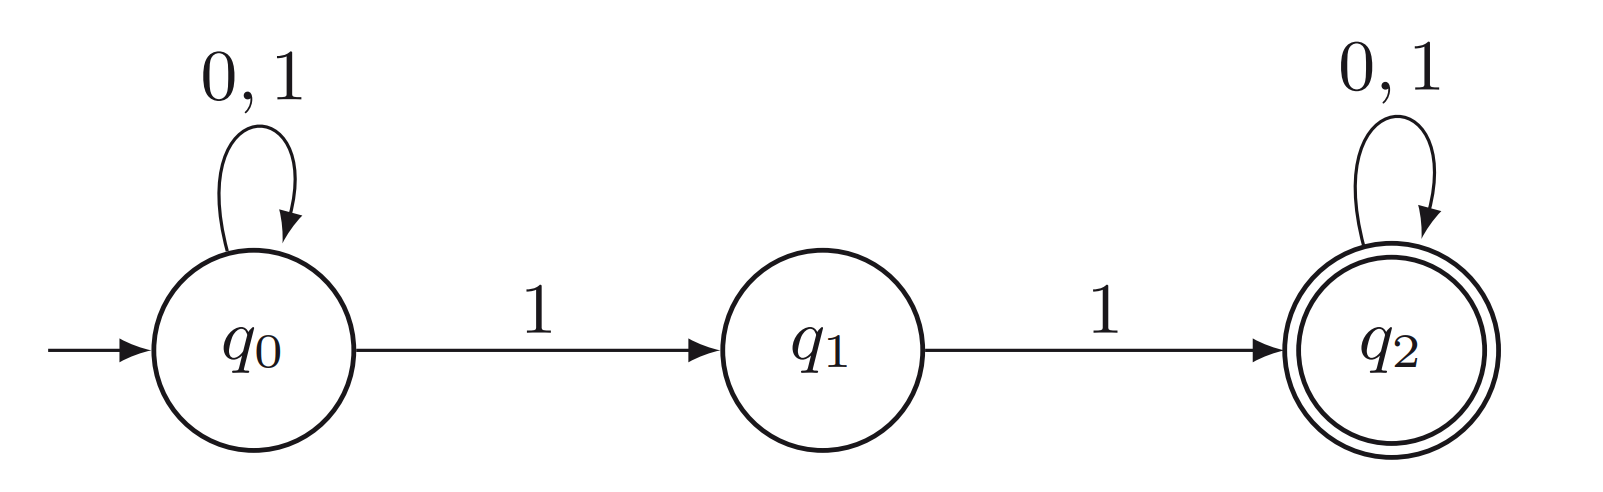
\includegraphics[width=0.8\textwidth]{Images/Beispiel_NEA.png}
            \caption[]{Abb. 3.15 aus dem Buch}
        \end{figure}
    
        \myTitle{Berechnungsbaum}

        Für ein Wort $x \in (\Sigma_{\text{bool}})^*$ ist ein Berechnungsbaum $\mathbf{\mathcal{B}_M(x)}$ nützlich, um zu erkennen, ob  $x \in L(M)$.
    
        \begin{figure}[htp]
            \centering
            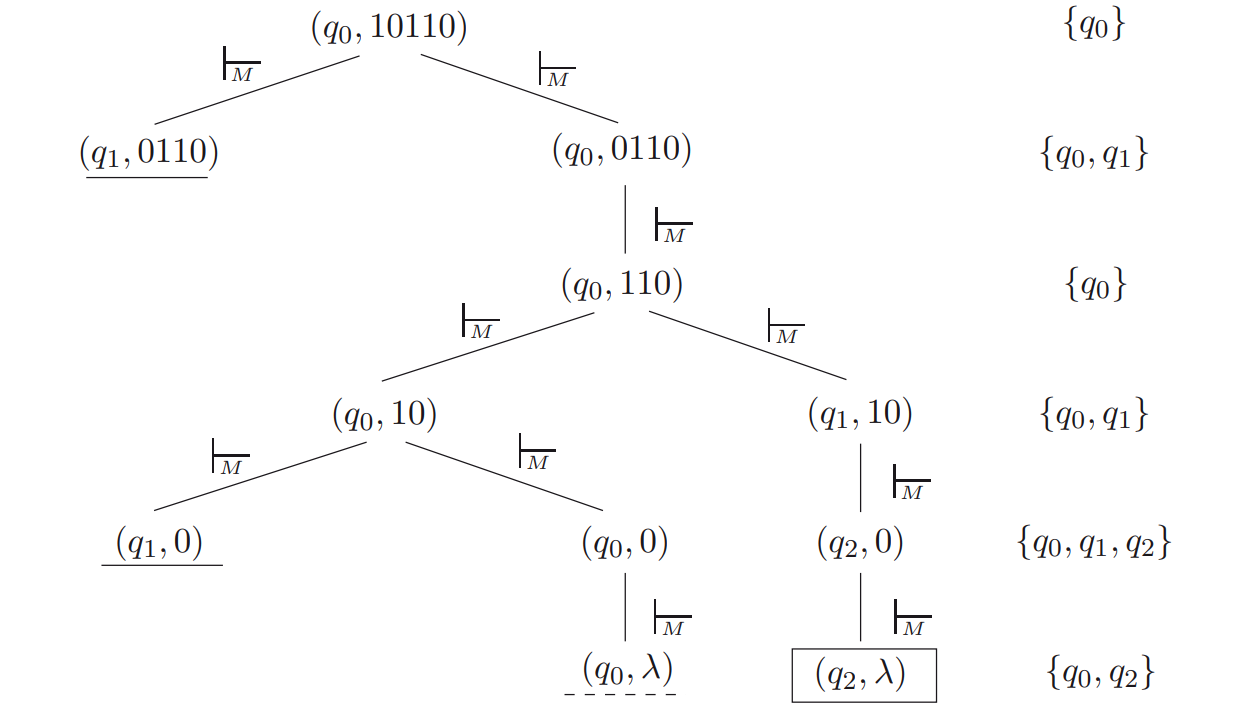
\includegraphics[width=0.6\textwidth]{Images/Berechnungsbaum.png}
            \caption{Abb. 3.16 aus dem Buch}
        \end{figure}
    
        Wir können die Sprache des NEA bestimmen.
        \begin{subbox}{Lemma 3.5}
            $$L(M) = \{x11y \mid x,y \in (\Sigma_{\text{bool}})^*\}$$
        \end{subbox}
        \textbf{Beweisidee}
    
        Beide Inklusionen zeigen und fertig. (Siehe Buch)
    
        Wir definieren die Klasse $\mathbf{\mathcal{L}_{\text{NEA}}}$.
        \begin{mainbox}{}
            $$\mathbf{\mathcal{L}_{\text{NEA}}} = \{L(M) \mid M \text{ ist ein NEA}\}$$
        \end{mainbox}
    
    
    
        \subsection{Äquivalenz von NEA und EA}
        Beweis von $\mathbf{\mathcal{L}_{\text{NEA}}} = \mathbf{\mathcal{L}_{\text{EA}}}$ per \textbf{Potenzmengenkonstruktion}.
        \begin{mainbox}{Satz 3.2}
            Zu jedem NEA $M$ existiert ein EA $A$, so dass
            $$L(M) = L(A)$$
        \end{mainbox}
        \textbf{Beweisidee}
    
        Potenzmengenkonstruktion und dann Induktion auf der Länge von einem Input i.e. $|x|$. (Siehe Buch)
    
    
    
        \textbf{Potenzmengenkonstruktion}
        \begin{subbox}{}
            Sei $M = (Q, \Sigma, \delta_M, q_0, F)$ ein NEA. Wir konstrurieren einen äquivalenten Endlichen Automaten $A = (Q_A, \Sigma_A, \delta_A, q_{0A}, F_A)$.
            \begin{enumerate}[label = (\roman*)]
                \item $Q_A = \{\langle P \rangle \mid P \subseteq Q\}$
                \item $\Sigma_A = \Sigma$
                \item $q_{0A} = \langle\{q_0\}\rangle$
                \item $F_A = \{\langle P\rangle \mid P \subseteq Q \text{ und } P \cap F \neq \emptyset\}$
                \item $\delta_A: (Q_A \times \Sigma_A) \to Q_A$ ist eine Funktion, definiert wie folgt. Für  jedes $\langle P \rangle \in Q_A$ und jedes $a \in \Sigma_A$ ist 
                \begin{align*}
                    \delta_A(\langle P \rangle, a) &= \left\langle \bigcup_{p \in P} \delta_M(p, a) \right\rangle\\
                    &= \left\langle\{q \in Q \mid \exists p \in P, \text{ so dass }q \in \delta_{M}(p, a)\}\right\rangle
                \end{align*}
            \end{enumerate}
        \end{subbox}
    
        \begin{figure}[htp]
            \centering
            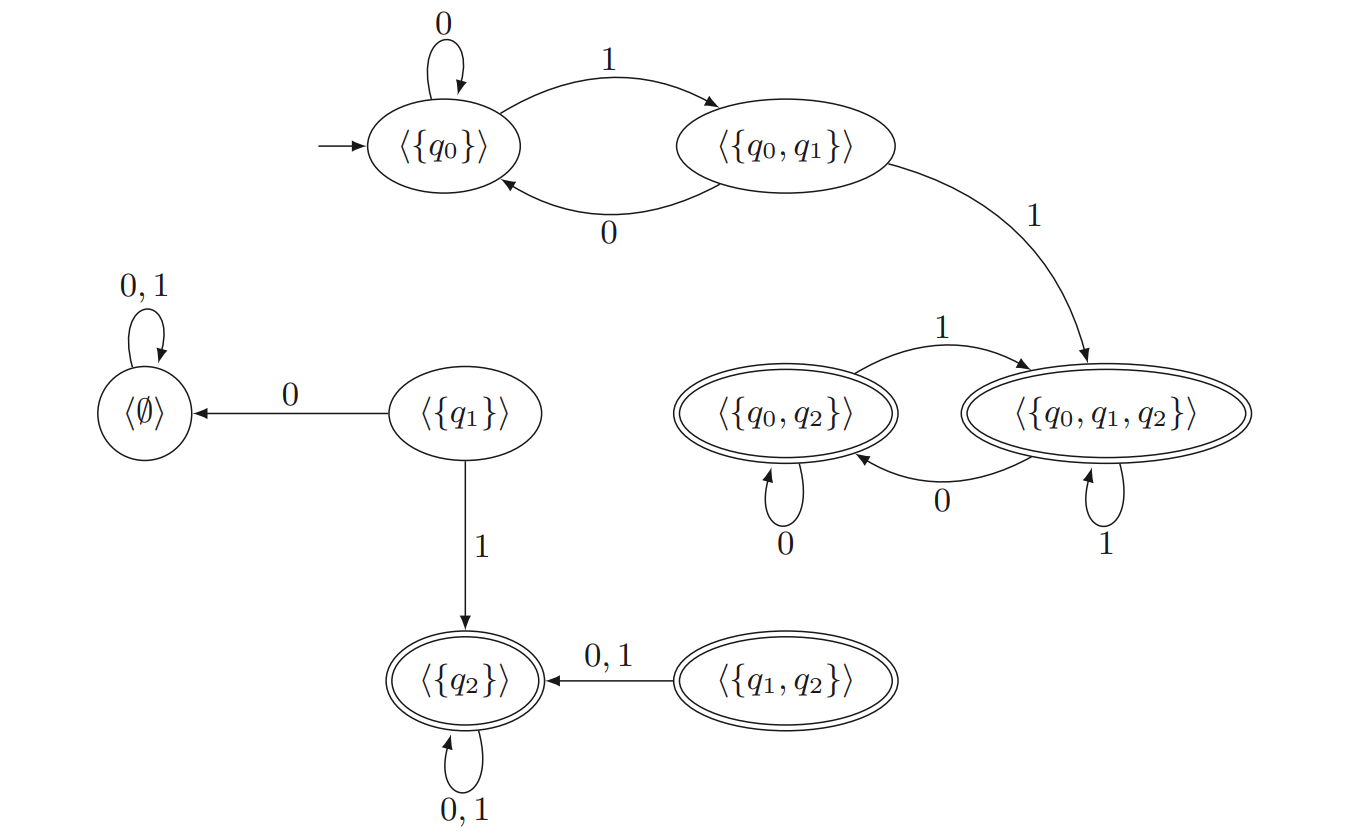
\includegraphics[width=0.75\textwidth]{Images/Potenzmengenkonstruktion_Beispiel.png}
            \caption{Abb. 3.18 im Buch}
        \end{figure}
    
    
    
        \subsection{Exponentiell mehr Zustände - manchmal}
        Sei 
        $$L_k = \{x1y \mid x \in (\Sigma_{\text{bool}})^*, \ y \in (\Sigma_{\text{bool}})^{k-1}\}$$
        Folgender NEA $A_k$ mit $k+1$ akzeptiert $L_k$.
        \begin{figure}
            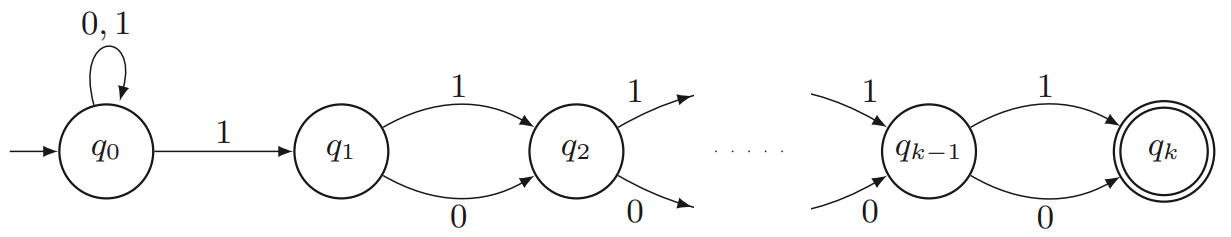
\includegraphics[width=0.8\textwidth]{Images/NEA_A_k.png}
            \caption{Abb. 3.19 im Buch}
        \end{figure}
    
        \begin{mainbox}{Lemma 3.6}
            Für alle $k \in \N \setminus \{0\}$ muss jeder EA, der $L_k$ akzeptiert, mindestens $2^k$ Zustände haben.
        \end{mainbox}
        \textbf{Beweis}
    
        Sei $B_k = (Q_k, \Sigma_{bool}, \delta_k, q_{0k}, F_k)$ ein EA mit $L(B_k) = L_k$. 
        
        Nach \textbf{Lemma 3.3} gilt für $x,y \in (\Sigma_{bool})^*$:
    
        Wenn $\hat{\delta}_k (q_{0k}, x) = \hat{\delta}_k (q_{0k}, y)$, dann gilt für alle $z \in (\Sigma_{bool})^*$:
        $$xz \in L(B_k) \iff yz \in L(B_k)$$
    
        Die Idee des Beweises ist es, eine Menge $S_k$ von Wörtern zu finden, so dass für keine zwei unterschiedlichen Wörter $x, y \in S_k$ die Gleichung $\hat{\delta}_k (q_{0k}, x) = \hat{\delta}_k (q_{0k}, y)$ gelten darf. 
        Dann müsste $B_k$ mindestens $|S_k|$ viele Zustände haben.
        
    
        Wir wählen $S_k = (\Sigma_{bool})^k$ und zeigen, dass $\hat{\delta}_k(q_{0k}, u)$ paarweise unterschiedliche Zustände für alle $u \in  S_k$ sind. 
    
        Wir beweisen dies per Widerspruch. 
    
        Seien $x = x_1x_2...x_k$ und $y = y_1y_2...y_k$ für $x_i,y_i \in \Sigma_{bool}, i \in \{1, ..., k\}$ zwei unterschiedliche Wörter aus $S_k$.
    
        Nehmen wir zum Widerspruch an, dass $\hat{\delta}_k(q_{0k}, x) = \hat{\delta}_k(q_{0k}, y)$.
        
    
        Weil $x \neq y$, existiert ein $j \in \{1, ...,k\}$, so dass $x_j \neq y_j$. O.B.d.A. setzen wir $x_j = 1$ und $y_j = 0$. 
        Betrachten wir nun $z = 0^{j-1}$.  Dann ist 
    
        $xz = x_1...x_{j-1}1x_{j+1}...x_k0^{j-1}$ und $yz = y_1...y_{j-1}0y_{j+1}...y_k0^{j-1}$
    
        und daher $xz \in L_k$ und $yz \notin L_k$. 
        
        Dies ist ein Widerspruch! Folglich gilt $\hat{\delta}_k(q_{0k}, x) \neq \hat{\delta}_k(q_{0k}, y)$ für alle paarweise unterschiedliche $x,y \in S_k = (\Sigma_{bool})^k$.
        
        Daher hat $B_k$ mindestens $|S_k| = 2^k$ viele Zustände.
        
        \hspace*{0pt}\hfill$\blacksquare$
    
    
    \subsection{Mindestanzahl Zustände}
    
        Die Grundidee ist es $n$ Wörter anzugeben und zu beweisen, dass jedes von diesen $n$ Wörtern in einem eigenen Zustand enden muss.
        
        Seien $w_1, ...,w_n$ diese Wörter. Dann geben wir für jedes Paar von Wörtern $w_i \neq w_j$ einen Suffix $z_{i,j}$ an, so dass folgendes gilt:
        $$w_iz_{i,j} \in L \centernot{\iff} w_jz_{i,j} \in L$$
        Dann folgt aus Lemma 3.3
        $$\hat{\delta}(q_0, w_i) \neq \hat{\delta}(q_0, w_j)$$
        
        Es eignet sich die Suffixe als Tabelle anzugeben.
    
        Um die Wörter und Suffixe zu finden, kann es sich als nützlich erweisen, den Endlichen Automaten zu konstruieren.
    
    
    
        \myTitle{Beweisschema}

        Wir nehmen zum Widerspruch an, dass es einen EA für $L$ gibt mit weniger als $n$ Zuständen.
    
        Betrachten wir $w_1, ...,w_n$. Per Pigeonhole-Principle existiert $i < j$, so dass
        $$\hat{\delta}(q_0, w_i) = \hat{\delta}(q_0, w_j)$$
        Per Lemma 3.3 folgt daraus, dass 
        $$\forall z \in \Sigma^*: w_iz \in L \iff w_jz \in L$$
        Für $z = z_{i,j}$ gilt aber per Tabelle $$w_iz_{i,j} \in L \centernot{\iff} w_jz_{i,j} \in L \quad \mathbf{(1)}$$ für alle $i< j$. 
        
        Da keines der $n$ Wörter im gleichen Zustand enden kann, ergibt sich ein Widerspruch.
    
        Dann noch Angabe der Tabelle für $\mathbf{(1)}$
        \begin{table}
            \centering
            \begin{tabular}{c|ccc}
                & $w_2$ & $...$ & $w_n$\\
                \hline
                $w_1$& $z_{1,2}$& ...&$z_{1,n}$\\
                $...$&  & $...$&$...$\\
                $w_{n-1}$& &  & $z_{n-1, n}$
            \end{tabular}
        \end{table}
        \begin{itemize}[label=-]
            \item Wenn es offensichtlich ist, muss $\mathbf{(1)}$ nicht bei jedem Suffix begründet werden.
            \item Ein minimaler endlicher Automat ist nicht notwendig für den Beweis. Hilft aber fürs
            \begin{enumerate}[label=\roman*.]
                \item Finden der $w_i$
                \item Finden der $z_{i, j}$
                \item Beweis von $w_iz_{i,j} \in L \centernot{\iff} w_jz_{i,j} \in L$ (Leicht überprüfbar)
            \end{enumerate}
        \end{itemize}
    
    
    
        \myTitle{Klassische Aufgabe - HS19 Aufgabe 3.a}

        Wir betrachten die Sprache 
        $$L = \{x00y \mid x \in \{0, 1\}^* \text{ und } y \in \{0,1\}\}$$
       
        Konstruieren Sie einen nichtdeterminstischen endlichen Automaten mit höchstens $4$ Zuständen, der $L$ akzeptiert.
        
        \begin{tikzpicture}[shorten >=2pt,node distance=3.5cm,on grid,auto]
            \node[state,initial]    (q_0) {$q_0$};
            \node[state]            (q_1)  [right of=q_0] {$q_1$};
            \node[state]            (q_2)  [right of=q_1] {$q_2$};
            \node[state, accepting] (q_3)  [right of=q_2]    {$q_3$};
            \path[->]
            (q_0) edge [loop above] node {$0, 1$}   (   )
                  edge [bend left]  node {$0$}   (q_1)
            (q_1) edge [bend left]  node {$0$}   (q_2)
            (q_2) edge [bend left] node {$0, 1$}   (q_3)
            ;
        \end{tikzpicture}
    
    
    
        \myTitle{Klassische Aufgabe - HS19 Aufgabe 3.b}

        Zeigen Sie, dass jeder deterministische endliche Automat, der $L$ akzeptiert, mindestens $5$ Zustände braucht.
        
        
        Wir zeichnen den zugehörigen EA zuerst.

        \begin{tikzpicture}[shorten >=2pt,node distance=3cm,on grid,auto]
            \node[state,initial]    (q_0) {$q_0$};
            \node[state]            (q_1)  [right of=q_0] {$q_1$};
            \node[state]            (q_2)  [right of=q_1] {$q_2$};
            \node[state, accepting] (q_3)  [above right of=q_2]    {$q_3$};
            \node[state, accepting] (q_4) [below right of=q_2] {$q_4$};
            \path[->]
            (q_0) edge [loop above] node {$1$}   (   )
                  edge [bend left]  node {$0$}   (q_1)
            (q_1) edge [bend left]  node {$0$}   (q_2)
                  edge [bend left]  node {$1$}   (q_0)
            (q_2) edge [bend left]  node {$0$}   (q_3)
                  edge [bend right] node {$1$}   (q_4)
            (q_3) edge [loop right] node {$0$}   (   )
                  edge [bend left] node {$1$}   (q_4)
            (q_4) edge [bend left]  node {$0$}   (q_1)
                  edge [bend left]  node {$1$}   (q_0)   
            ;
        \end{tikzpicture}
    
        Nehmen wir zum Widerspruch an, dass es einen endlichen Automaten gibt, der $L$ akzeptiert und weniger als $4$ Zustände hat.
    
        Wir wählen die Wörter $B = \{\lambda, 0, 00, 000, 001\}$.
    
        Nach dem Pigeonhole-Principle existieren zwei Wörter $w_i, w_j \in B, w_i \neq w_j$, so dass 
        $$\hat{\delta}(q_0, w_i) = \hat{\delta}(q_0, w_j)$$
        Per Lemma 3.3 folgt daraus, dass 
        $$\forall z \in \Sigma^*: w_iz \in L \iff w_jz \in L$$
        
        Wir betrachten folgende Tabelle mit Suffixen.
        \begin{table}[htp]
            \centering
            \begin{tabular}{c|cccc}
                          & $0$  & $00$& $000$     & $001$    \\
                \hline
                $\lambda$ & $01$ & $1$ & $\lambda$ & $\lambda$\\
                $0$       &      & $1$ & $\lambda$ & $\lambda$\\
                $00$      &      &     & $\lambda$ & $\lambda$ \\
                $000$     &      &     &           & $1$ 
            \end{tabular}
        \end{table}
        Der zeigt für jedes Wortpaar $x, y \in B, x \neq y$ die Existenz eines Suffixes $z$, so dass 
        $$\left(xz \in L \land yz \notin L\right) \lor \left(xz \notin L \land yz \in L\right)$$
        Dies kann man mit den angegebenen Suffixen und dem angegebenen EA einfach überprüfen.
    
        Dies widerspricht der vorigen Aussage, dass ein Wortpaar $w_i, w_j \in B, w_i \neq w_j$ existiert, so dass
        $$\forall z \in \Sigma^*: w_iz \in L \iff w_jz \in L$$
        Somit ist unsere Annahme falsch und ein EA für $L$ muss mindestens $4$ Zustände haben.
    
        $\hfill\blacksquare$
    
        \textbf{Bemerkung}

        Manchmal ist es zu schwierig einen minimalen EA zu finden und es funktioniert einfacher die Wörter durch Trial and Error zu finden. (Siehe Midterm HS22)
    
    
    
    \section{Turing Maschinen}
    
    
        \subsection{Motivation und Überblick}
        Formalisierung notwendig, um mathematisch über die automatische Unlösbarkeit zu argumentieren.
    
        Jede vernünftige Programmiersprache ist eine zulässige Formalisierung. 
    
        Aber nicht geeignet (meistens komplexe Operationen).
    
        Die Turingmaschine erlaubt ein paar \textbf{elementare Operationen} und besitzt trotzdem die \textbf{volle Berechnungsstärke} beliebiger Programmiersprachen.
    
        Ziel dieses Kapitels ist, dass ihr ein gewisse Gespür dafür bekommt, was eine Turingmaschine kann und was nicht.
    
    
    
        \subsection{Turing Maschinen - Formalisierung von Algorithmen}
        \begin{subbox}{Informell}
            Eine Turingmaschine besteht aus 
            \begin{enumerate}[label=(\roman*)]
                \item einer endlichen Kontrolle, die das Programm enthält,
                \item einem unendlichen Band, das als Eingabeband, aber auch als Speicher (Arbeitsband) zur Verfügung steht, und 
                \item einem Lese-/Schreibkopf, der sich in beiden Richtungen auf dem Band bewegen kann.
            \end{enumerate}
        \end{subbox}
        Für formale Beschreibung siehe Buch.
    
        \begin{figure}[htp]
            \centering
            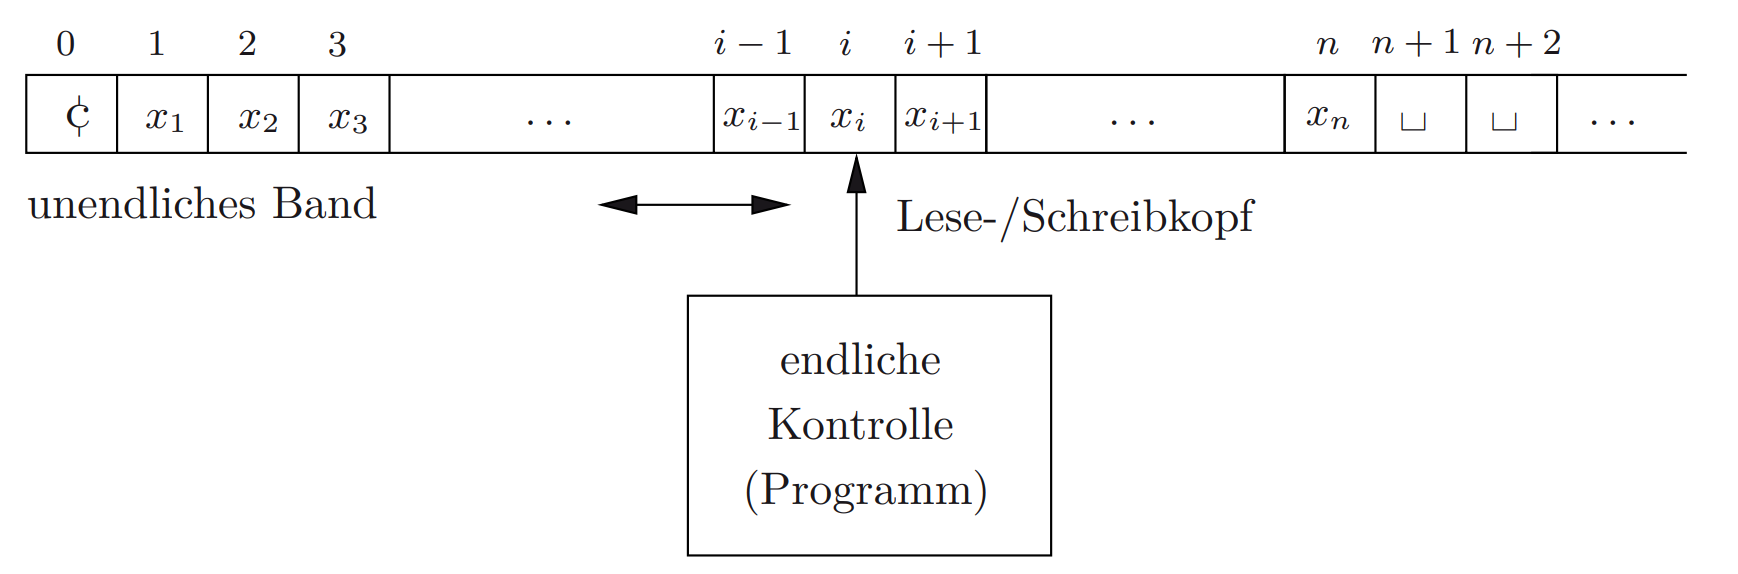
\includegraphics[width=0.7\textwidth]{Images/Turingmaschine.png}
            \caption{Abb. 4.1 vom Buch}
        \end{figure}
    
        \begin{mainbox}{Elementare Operation einer TM - Informell}
            \textbf{Input}
            \begin{itemize}[label = -]
                \item Zustand der Maschine (der Kontrolle)
                \item Symbol auf dem Feld unter dem Lese-/Schreibkopf
            \end{itemize}
            \textbf{Aktion}
            \begin{enumerate}[label=(\roman*)]
                \item ändert Zustand
                \item schreibt auf das Feld unter dem Lese-/Schreibkopf
                \item bewegt den Lese-/Schreibkopf nach links, rechts oder gar nicht. Ausser wenn $\cent$, dann ist links nicht möglich.
            \end{enumerate}
        \end{mainbox}
    
        \begin{mainbox}{}
            Eine \textbf{Konfiguration $C$} von $M$ ist ein Element aus 
            $$\textbf{Konf($\mathbf{M}$)} =  \{\cent\} \cdot \Gamma^* \cdot Q \cdot \Gamma^+ \cup Q \cdot \{\cent\} \cdot \Gamma^*$$
        \end{mainbox}
        \begin{itemize}[label=-]
            \item Eine Konfiguration $\cent w_1qaw_2$ mit $w_1, w_2 \in \Gamma^*$, $a \in \Gamma$ und $q \in Q$ sagt uns:
            
            $M$ im Zustand $q$, Inhalt des Bandes $\cent w_1aw_2 \text{\textvisiblespace} \text{\textvisiblespace} \text{\textvisiblespace}...$, Kopf an Position $|w_1|+1$ und liest gerade $a$.
            \item Eine Konfiguration $p\cent w$ mit $p \in Q$, $w\in \Gamma^*$: Inhalt des Bandes $\cent w \text{\textvisiblespace}  \text{\textvisiblespace}  \text{\textvisiblespace}...$, Zustand $p$ und Kopf an Position $0$. 
        \end{itemize}
        Bmk: Im Buch haben sie in der Definition von Konf $\Gamma^+$ anstatt $\Gamma^*$ an ''letzter Stelle''.
    
        Es gibt wieder eine Schrittrelation $\sststile{M}{} \subseteq \text{Konf}(M) \times \text{Konf}(M)$.
    
        \begin{figure}[htp]
            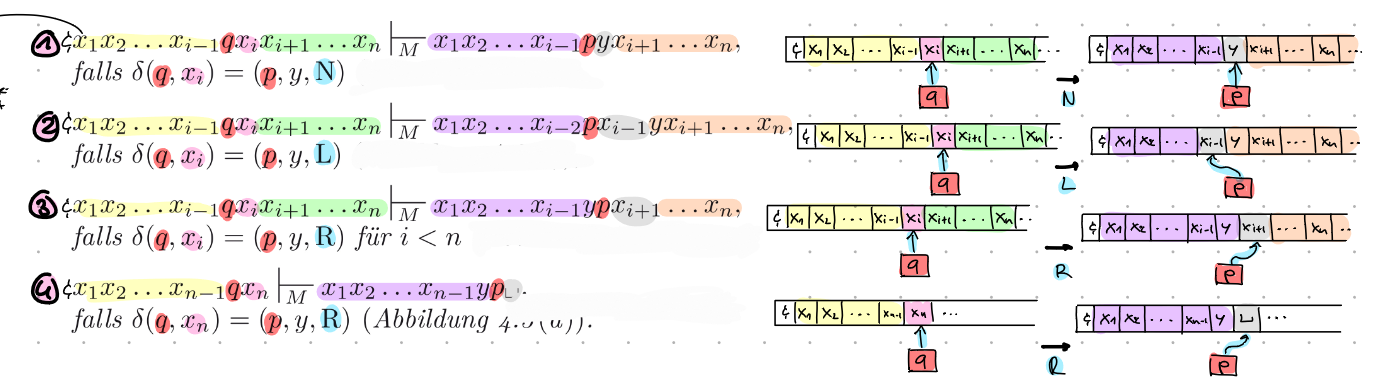
\includegraphics[width=\textwidth]{Images/Schrittrelation.png}
            \caption{Diagramm von Adeline}
        \end{figure}
    
        \textbf{Berechnung von $\mathbf{M}$}, \textbf{Berechnung von $\mathbf{M}$ auf einer Eingabe $\mathbf{x}$} etc. durch $\sststile{M}{}$ definiert.
    
        \begin{mainbox}{}
            Die Berechnung von $M$ auf $x$ heisst 
            \begin{itemize}[label=-]
                \item \textbf{akzeptierend}, falls sie in einer akzeptierenden Konfiguration $w_1q_{\text{accept}}w_2$ endet (wobei $\cent$ in $w_1$ enthalten ist).
                \item \textbf{verwerfend}, wenn sie in in einer verwerfenden Konfiguration $w_1q_{\text{reject}}w_2$ endet.
                \item \textbf{nicht-akzeptierend}, wenn sie entweder eine \textbf{verwerfende} oder unendliche Berechnung ist.
            \end{itemize}
        \end{mainbox}
    
        \begin{mainbox}{}
            Die von der \textbf{Turingmaschine $\mathbf{M}$ akzeptierte Sprache} ist 
            $$\mathbf{L(M)} = \{w \in \Sigma^* \mid q_0\cent w \sststile{M}{*}yq_{\text{accept}}z, \text{ für irgendwelche }y, z \in \Gamma^*\}$$
        \end{mainbox}
    
    
    
        \subsection{Wichtige Klassen}
        \begin{subbox}{Reguläre Sprachen}
            $$\mathbf{\mathcal{L}_{\textbf{EA}}} = \{L(A) \mid A \text{ ist ein EA}\} = {\mathcal{L}_{\textbf{NEA}}}$$
        \end{subbox}
    
        \begin{mainbox}{Rekursiv aufzählbare Sprachen}
            Eien Sprache $L \subseteq \Sigma^*$ heisst \textbf{rekursiv aufzählbar}, falls eine TM $M$ existiert, so dass $L = L(M)$.
            $$\mathbf{\mathcal{L}_{\textbf{RE}}} = \{L(M) \mid M \text{ ist eine TM}\}$$
            ist die \textbf{Klasse aller rekursiv aufzählbaren Sprachen}.
        \end{mainbox}
    
        \begin{subbox}{Halten}
            Wir sagen das $M$ \textbf{immer hält}, wenn für alle Eingaben $x \in \Sigma^*$
            \begin{enumerate}[label=(\roman*)]
                \item $q_0\cent x \sststile{M}{*} yq_{\text{accept}}z, y,z \in \Gamma^*, \text{ falls }x \in L \text{ und }$
                \item $q_0 \cent x \sststile{M}{*} uq_{\text{reject}}v, u,v \in \Gamma^*, \text{ falls }x \notin L.$
            \end{enumerate}
        \end{subbox}
    
        \begin{mainbox}{Rekusive Sprachen}
            Eine Sprache $L \subseteq \Sigma^*$ heisst \textbf{rekursiv (entscheidbar)}, falls $L = L(M)$ für eine TM $M$, die \textbf{immer hält}.
            $$\mathbf{\mathcal{L}_{\textbf{R}}} = \{L(M) \mid M \text{ ist eine TM, die immer hält}\}$$
            ist die \textbf{Klasse der rekursiven (algorithmisch erkennbaren) Sprachen}.
        \end{mainbox}
    
    
    
        \subsection{Mehrband-Turingmaschine}
        \begin{mainbox}{Mehrband-TM - Informelle Beschreibung}
            Für $k \in \N\setminus\{0\}$ hat eine $k$-Band Turingmaschine 
            \begin{itemize}[label=-]
                \item eine endliche Kontrolle 
                \item ein endliches Band mit einem Lesekopf (Eingabeband)
                \item $k$ Arbeitsbänder, jedes mit eigenem Lese-/Schreibkopf (nach rechts unendlich)
            \end{itemize}
        \end{mainbox}
        \textbf{Insbesondere gilt $1$-Band TM $\neq$ ''normale'' TM}
    
        Am Anfang der Berechnung einer MTM $M$ auf $w$
        \begin{itemize}[label=-]
            \item Arbeitsbänder ''leer'' und die $k$ Lese-/Schreibköpfe auf Position $0$.
            \item Inhalt des Eingabebands $\cent w \$$ und Lesekopf auf Position $0$.
            \item Endliche Kontrolle im Zustand $q_0$.
        \end{itemize}
    
    
    
        \subsection{Äquivalenz von Maschinen (TM, MTM)}
        \begin{mainbox}{}
            Seien $A$ und $B$ zwei Maschinen mit \textbf{gleichem} $\Sigma$.
    
            Wir sagen, dass \textbf{$\mathbf{A}$ äquivalent zu $\mathbf{B}$ ist}, wenn für jede Eingabe $x \in \Sigma^*$
            \begin{enumerate}[label=(\roman*)]
                \item $A$ akzeptiert $x$ $\iff$ $B$ akzeptiert $x$
                \item $A$ verwirft $x$ $\iff$ $B$ verwirft $x$
                \item $A$ arbeitet unendlich lange auf $x$ $\iff$ $B$ arbeitet unendlich lange auf $x$
            \end{enumerate}
        \end{mainbox}
        Wir haben 
        \begin{center}
            $A$ und $B$ äquivalent $\implies$ $L(A) = L(B)$
    
            aber 
    
            $L(A) = L(B)$ $\centernot{\implies}$ $A$ und $B$ äquivalent
        \end{center}
        da $A$ auf $x$ unendlich lange arbeiten könnte, während $B$ $x$ verwirft.
    
        \begin{mainbox}{Lemma 4.1}
            Zu jeder TM $A$ existiert eine zu $A$ äquivalente 1-Band-TM $B$
        \end{mainbox}
        \textbf{Beweisidee}
        $B$ kopiert die Eingabe zuerst aufs Arbeitsband und simuliert dann $A$.
    
        \begin{mainbox}{Lemma 4.2}
            Zu jeder Mehrband-TM $A$ existiert eine zu $A$ äquivalente TM $B$
        \end{mainbox}
        \textbf{Beweis}
        
        Sei $A$ eine $k$-Band-Turingmaschine für ein $k \in \N \setminus \{0\}$. Wir konstruieren eine TM $B$, die Schritt für Schritt $A$ simuliert.

        $B$ speichert die Inhalte aller $k+1$ Bänder von $A$ auf ihrem einzigen Band. Anschaulich gesprochen ist jedes Feld auf dem Band von $B$ ein $2(k+1)$-Tupel und jedes Element dieses Tupels ist auf einer Spur. 
        Sei $\Gamma_A$ das Arbeitsalphabet von $A$. Dann gilt 
        $$\Gamma_B = (\Sigma_A \cup \{\cent, \$, \text{\textvisiblespace}\}) \times \{\text{\textvisiblespace},\uparrow\} \times (\Gamma_A \times \{\text{\textvisiblespace}, \uparrow\})^k \cup \Sigma_A \cup \{\text{\textvisiblespace}, \cent\}$$
        Für ein Symbol $\alpha = (a_0,a_1,a_2,...,a_{2k+1}) \in \Gamma_B$ sagen wir, dass $a_i$ auf der $i$-ten Spur liegt. Daher bestimmen die $i$-ten Elemente der Symbole auf dem Band von $B$ den Inhalt der $i$-ten Spur. Eine Konfiguration $(q,w,i,x_1,i_1,x_2,i_2,...,x_k,i_k)$ von $A$ ist dann in $B$ wie folgt gespeichert. 
        \begin{itemize}
            \item Der Zustand $q$ ist in der endlichen Kontrolle von $B$ gespeichert. 
            \item Die $0$-te Spur des Bandes von $B$ enthält die $\cent w\$$ (i.e. den Inhalt des Eingabebandes von $A$)
            \item Für alle $i \in \{1, ..., k\}$ enthält die $(2i)$-te Spur des Bandes von $B$ den Inhalt vom $i$-ten Band von $A$ (i.e. $\cent x_i\$$).
            \item Für alle $i \in \{1, ..., k\}$ bestimmt die $(2i +1)$-te Spur des Bandes von $B$ mit dem Symbol $\uparrow$ die Position des Kopfes auf dem $i$-ten Arbeitsband von $A$.
        \end{itemize}
        Ein Schritt von $A$ kann jetzt durch folgende Prozedur von $B$ simuliert werden:
        \begin{enumerate}
            \item $B$ liest einmal den Inhalt ihres Bandes von links nach rechts, bis sie alle $k+1$ Kopfpositionen von $A$ gefunden hat, und speichert dabei in ihrem Zustand die $k+1$ Symbole, die an diesen Positionen stehen. (Dies kann ohne weiteres in der Zustandsmenge abgespeichert werden, da $k$ fix ist, folglich ist dann $\Gamma_A^k$ auch endlich)
            \item Nach der ersten Phase kennt $B$ das ganze Argument (der Zustand von $A$ ist im Zustand von $B$ gespeichert) der Transitionsfunktion von $A$ und kann also die entsprechenden Aktionen (Köpfe bewegen, Ersetzen von Symbolen) von $A$ bestimmen. Diese Änderungen führt $B$ in einem Lauf über ihr Band von rechts nach links durch.
        \end{enumerate}
        \hspace*{0pt}\hfill$\blacksquare$
    
        Aus Lemma 4.1 und 4.2 folgt direkt
        \begin{mainbox}{Satz 4.1}
            Die Maschinenmodelle von Turingmaschinen und Mehrband-Turingmaschinen sind äquivalent.
        \end{mainbox}
        Note: 
        \begin{itemize}
            \item ''Äquivalenz'' für Maschinenmodelle wird in Definition 4.2 definiert.
            \item Maschinenmodelle sind Klassen von Maschinen (i.e. Mengen von Maschinen mit gewissen Eigenschaften).
        \end{itemize}
    
        \subsection{Nichtdeterministische Turingmaschinen}
            \begin{mainbox}{Definition von NTM}
                Eine \textbf{nichtdeterministische Turingmaschine (NTM)} ist ein $7$-Tupel $M = (Q, \Sigma, \Gamma, \delta, q_0, q_{\text{accept}}, q_{\text{reject}})$, wobei 
                \begin{enumerate}[label=(\roman*)]
                    \item $Q, \Sigma, \Gamma, q_{\text{accept}}, q_{\text{reject}}$ die gleiche Bedeutung wie bei einer TM haben, und
                    \item $\delta: (Q \setminus \{q_{\text{accept}}, q_{\text{reject}}\}) \times \Gamma \to \mathcal{P}(Q \times \Gamma \times \{\text{L, R, N}\})$ 
                    die \textbf{Übergangsfunktion} von $M$ ist und die folgende Eigenschaft hat:
                    $$\delta(p, \cent) \subseteq \{(q, \cent, X) \mid q \in Q, X \in \{R, N\}\}$$
                    für alle $p \in Q$
                \end{enumerate}
            \end{mainbox}
            \textbf{Konfiguration} ähnlich wie bei TMs.
            \begin{center}
                Konfiguration akzeptierend $\iff$ enthält $q_{\text{accept}}$\\
                Konfiguration verwerfend $\iff$ enthält $q_{\text{reject}}$
            \end{center}
        
        
        
            \textbf{Die üblichen Sachen}
            \begin{itemize}[label=-]
                \item Schrittrelation $\sststile{M}{}$ ''verbindet zwei Konfigurationen, wenn man von der einen in die andere kommen kann''
                \item Reflexive und transitive Hülle ist $\sststile{M}{*}$.
                \item Berechnung von $M$ ist eine Folge von Konfigurationen $C_1, C_2, ...$, so dass $C_i \sststile{M}{} C_{i+1}$.
                \item Eine Berechnung von $M$ auf $x$ ist beginnt in $q_0\cent x$ und endet entweder unendlich oder endet in $\{q_{\text{accept}}, q_{\text{reject}}\}$.
            \end{itemize}
            \begin{mainbox}{Akzeptierte Sprache}
                $$L(M) = \{w \in \Sigma^* \mid q_0\cent w \sststile{M}{*} yq_{\text{accept}}z \text{ für irgendwelche }y,z \in \Gamma^*\}$$
            \end{mainbox}
        
        
        
            \textbf{Berechnungsbaum}
            \begin{mainbox}{}
                Sei $M=  (Q, \Sigma, \Gamma, \delta, q_0, q_{\text{accept}}, q_{\text{reject}})$ eine NTM 
                und sei $x$ ein Wort über dem Eingabealphabet $\Sigma$ von $M$. 
                Ein \textbf{Berechnungsbaum $\mathbf{T_{M, x}}$ von $\mathbf{M}$ auf $\mathbf{x}$} ist ein 
                (potentiell unendlicher) gerichteter Baum mit einer Wurzel, der wie folgt definiert wird.
        
                \begin{enumerate}[label=(\roman*)]
                    \item Jeder Knoten von $T_{M,x}$ ist mit einer Konfiguration beschriftet.
                    \item Die Wurzel ist der einzige Knoten von $T_{M,x}$ mit dem Eingangsgrad $0$ und ist mit der Startkonfiguration $q_0\cent x$ beschriftet.
                    \item Jeder Knoten des Baumes, der mit einer Konfiguration $C$ beschriftet ist, hat genauso viele Kinder wie $C$ Nachfolgekonfigurationen hat, und diese Kinder sind mit diesen Nachfolgekonfigurationen $C$ markiert.
                \end{enumerate}
            \end{mainbox}
        
        
        
            \textbf{Äquivalenz NTM und TM}
            \begin{mainbox}{Satz 4.2}
                Sei $M$ eine NTM. Dann existiert eine TM $A$, so dass 
                \begin{enumerate}[label=(\roman*)]
                    \item $L(M) = L(A)$ und 
                    \item falls $M$ keine unendlichen Berechnungen auf Wörtern aus $L(M)^\complement$ hat, dann hält $A$ immer.
                \end{enumerate}
            \end{mainbox}
            \textbf{Beweisidee:} 
            
            ''BFS im Berechnungsbaum'', i.e. wir simulieren einzelne Schritte der verschiedenen Berechnungsstränge.
        
        
        \section{Einstieg Berechnenbarkeit}
        
        \subsection{Diagonalisierung}
        
        
            \textbf{Bijektion, Injektion, Schreibweise}
            \begin{mainbox}{}
                Seien $A$ und $B$ zwei Mengen.
        
                Wir sagen, dass 
                \begin{enumerate}[label=\roman*.]
                    \item $\mathbf{|A| \leq |B|}$, falls eine injektive Funktion $f: A \to B$ existiert.
                    \item $\mathbf{|A| = |B|}$, falls $|A| \leq |B|$ und $|B| \leq |A|$.
                    \item $\mathbf{|A| < |B|}$, falls $|A| \leq |B|$ und keine injektive Abbildung von $B$ nach $A$ existiert.
                \end{enumerate}
            \end{mainbox}
            \textbf{Zur Erinnerung:}
            \begin{center}
                $f: A \to B$ injektiv $\iff $ $\forall x,y \in A, x\neq y. f(x) \neq f(y)$
            \end{center}
        
        
        
            \textbf{Abzählbarkeit}
            \begin{mainbox}
                Eine Menge $A$ heisst \textbf{abzählbar}, falls $A$ endlich ist oder $|A| = |\N|$.
            \end{mainbox}
            \begin{subbox}{Lemma 5.1}
            Sei $\Sigma$ ein beliebiges Alphabet. Dann ist $\Sigma^*$ abzählbar.
            \end{subbox}
            % \textbf{Beweisidee}
        
            % kanonische Ordnung gibt uns eine Bijektion zwischen $\N$ und $\Sigma^*$.
        
            \begin{mainbox}{Satz 5.1}
                Die Menge \textbf{KodTM} der Turingmaschinenkodierungen ist abzählbar.
            \end{mainbox}
            \textbf{Beweisidee}
        
            KodTM $\subseteq (\Sigma_{\text{bool}})^*$ und Lemma 5.1
        
            \begin{mainbox}{Lemma 5.2}
                $(\N\setminus\{0\}) \times (\N \setminus \{0\})$ ist abzählbar.
            \end{mainbox}
            \textbf{Beweisidee}
        
            Unendliche 2-dimensionale Tabelle, so dass an der $i$-ten Zeile und $j$-ten Spalte, sich das Element $(i,j) \in (\N\setminus\{0\}) \times (\N \setminus \{0\})$ befindet.
        
            Formal definiert man dabei die lineare Ordnung 
            $$(a,b) < (c,d) \iff a+b < c+d \text{ oder }(a+b = c+d \text{ und } b <d)$$
        
            \begin{figure}[htp]
                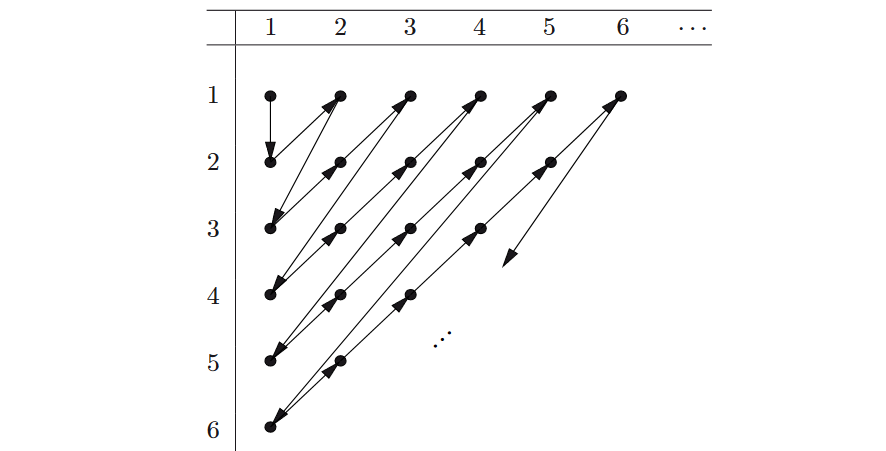
\includegraphics[width=0.7\textwidth]{Images/Abzählen.png}
                \caption{Abbildung 5.3 im Buch}
            \end{figure}
        
            Die $i$-te Diagonale hat $i$ Elemente. Ein beliebiges Element $(a,b) \in (\N\setminus\{0\}) \times (\N \setminus \{0\})$ ist das $b$-te Element auf der $(a+b-1)$-ten Diagonale.
            
            Auf den ersten $a+b-2$ Diagonalen gibt es 
            $$\sum_{i = 1}^{a+b-2}i = \frac{(a+b-2)\cdot((a+b-2)+1)}{2} = \binom{a+b-1}{2}$$
            Elemente.
        
            Folglich ist 
            $$f((a,b)) = \binom{a+b-1}{2} + b$$
            eine Bijektion von $(\N\setminus\{0\}) \times (\N \setminus \{0\})$ nach $\N\setminus\{0\}$.
        
        
        
            \textbf{Überabzählbarkeit}

            \begin{mainbox}{Satz 5.3}
                $[0,1]$ ist nicht abzählbar.
            \end{mainbox}
            \textbf{Beweisidee}
            
            Klassisches Diagonalisierungsargument. Aufpassen auf $0$ und $9$. I.e. $1 = 0.\overline{99}$.
        
            \begin{figure}[htp]
                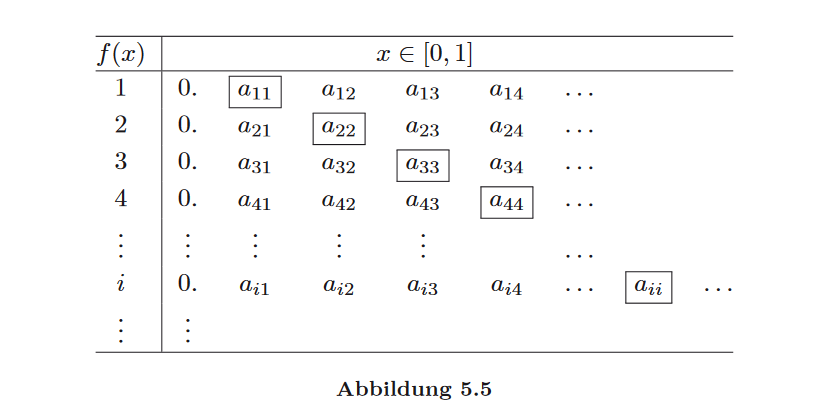
\includegraphics[width=0.7\textwidth]{Images/Diagonalisierung.png}
            \end{figure}
        
            \begin{mainbox}{Satz 5.4}
                $\mathcal{P}((\Sigma_{\text{bool}})^*)$ ist nicht abzählbar.
            \end{mainbox}
            \textbf{Beweis: }
        
                Wir definieren eine injektive Funktion von $f: [0, 1] \to \mathcal{P}((\Sigma_{bool})^*)$ und beweisen so $|\mathcal{P}((\Sigma_{bool})^*)| \geq |[0, 1]|$.
            
                Sei $a \in [0, 1]$ beliebig. Wir können $a$ wie folgt binär darstellen:
                $$\text{Nummer}(a) = 0.a_1a_2a_3a_4... \text{ mit } a = \sum_{i = 1}^{\infty} a_i\cdot 2^{-i}.$$ 
                
                Hier ist zu beachten, dass wir für eine Zahl $a$ immer die lexikographisch letzte Darstellung wählen.
            
            Dies tun wir, weil eine reelle Zahl 2 verschiedene Binärdarstellungen haben kann. Beispiel: $\frac{1}{2} = 0.1\overline{0} = 0.0\overline{1}$.
                
                Für jedes $a$ definieren wir:
                $$f(a) = \{a_1, a_2a_3, a_4a_5a_6, ..., a_{\binom{n}{2}+1}a_{\binom{n}{2}+2}...a_{\binom{n+1}{2}} , ...\}$$
            
                Da $f(a) \subseteq (\Sigma_{bool})^*$ gilt $f(a) \in \mathcal{P}((\Sigma_{bool})^*)$.
            
                Wir haben für alle $n \in \N \setminus\{0\}$, dass $f(a)$ \textbf{genau} ein Wort dieser Länge enthält. Nun können wir daraus folgendes schliessen:
            
                Weil die Binärdarstellung zweier unterschiedlichen reellen Zahlen an mindestens einer Stelle unterschiedlich ist, gilt $b \neq c \implies f(b) \neq f(c), \forall b,c \in [0, 1]$. 
            
                Folglich ist $f$ injektiv und wir haben $|\mathcal{P}((\Sigma_{bool})^*)| \geq |[0, 1]|$.
            
                Da $[0,1]$ nicht abzählbar ist, folgt daraus:
            
                $\mathcal{P}((\Sigma_{bool})^*)$ ist nicht abzählbar.
                
                \hspace*{0pt}\hfill$\blacksquare$
        
        
        
            \textbf{Diagonalsprache $L_{\text{diag}}$ }

            Zur Erinnerung:
            \begin{mainbox}{Rekursiv aufzählbare Sprachen}
                Eien Sprache $L \subseteq \Sigma^*$ heisst \textbf{rekursiv aufzählbar}, falls eine TM $M$ existiert, so dass $L = L(M)$.
                $$\mathbf{\mathcal{L}_{\textbf{RE}}} = \{L(M) \mid M \text{ ist eine TM}\}$$
                ist die \textbf{Klasse aller rekursiv aufzählbaren Sprachen}.
            \end{mainbox}
            Wir zeigen jetzt per Diagonalisierung, die Existenz einer Sprache die nicht rekursiv aufzählbar ist.
        
        
            Sei $w_1, w_2,...$ die kanonische Ordnung aller Wörter über $\Sigma_{\text{bool}}$ und sei $M_1, M_2, M_3,...$ die Folge aller Turingmaschinen.
            
            Wir definieren eine unendliche (bool'sche) Matrix $A = [d_{ij}]_{i,j = 1, 2, ...}$ mit 
            $$d_{ij} = 1 \iff M_i \text{ akzeptiert }w_j.$$
        
            Wir definieren
            $$L_{\text{diag}} = \{w \mid w = w_i \text{ und $M_i$ akzeptiert $w_i$ nicht für ein $i \in \N\setminus\{0\}$}\}$$
        
        
            \begin{mainbox}{Satz 5.5}
                $$L_{\text{diag}} \notin \L_{\text{RE}}$$
            \end{mainbox}
        
            \textbf{Beweis:}
        
            Wir haben 
            $$L_{\text{diag}} = \{w \mid w = w_i \text{ und $M_i$ akzeptiert $w_i$ nicht für ein $i \in \N\setminus\{0\}$}\}$$
        
            Widerspruchsbeweis:
        
            Sei $L_\text{diag} \in \L_{\text{RE}}$. Dann existiert eine TM $M$, so dass $L(M) = L_\text{diag}$. Da diese TM eine TM in der Nummerierung aller TM ist, existiert ein $i \in \N$, so dass $M_i = M$.
        
            Wir betrachten nun das Wort $w_i$ für diese $i \in \N$. Per Definition von $L_\text{diag}$, gilt:
        
            $$w_i \in L_\text{diag} \iff w_i \notin L(M_i)$$
        
            Da aber $L(M_i) = L_\text{diag}$, haben wir folgenden Widerspruch:
            $$w_i \in L_\text{diag} \iff w_i \notin L_\text{diag}$$
        
            Folglich gilt $L_\text{diag} \notin \L_\text{RE}$.
            
            \hspace*{0pt}\hfill$\blacksquare$
        
        
            
                \subsection{Klassifizierung verschiedener Sprachen}
                \begin{tikzpicture}
                    \draw (0,0) circle (3.75);
                    \draw (0,0) circle (2.5);
                    \draw (0,0) circle (1.25);
                    \node at (0, 3.25) {\Large$\mathcal{L}_{RE}$};
                    \node at (0, 2.) {\Large$\mathcal{L}_R$};
                    \node at (0, 0) {\Large$\mathcal{L}_{EA}$};
                    
                    % \node at (0, -0.25) {$\{|x|_a \mod 3 = 1\}$};
                    \node at (-0.25, -1.75) {$\{0^n1^n \,|\, n\in \mathbb{N}\}$};
                    \node at (-3.5, 3) {$L_\text{diag}$};
                    \node at (2.5, 2) {$L_{H}$};
                    \node at (-1.75, -2.75) {$L_U$};
                    \node at (3.75, -2.75) {$L_\text{empty}$};
                    \node at (3.75, 2.75) {$(L_H)^C$};
                    \node at (-1.5, 1.25) {$L_\text{prim}$};
                    
                \end{tikzpicture}
            
            
            
                \subsection{Begrifflichkeiten}

                Für eine Sprache $L$ gilt folgendes
                \begin{center}
                    $L$ regulär $\iff $ $L \in \mathbf{\mathcal{L}_{\textbf{EA}}}$ $\iff$ $\exists$ EA $A$ mit $L(A) = L$\\
                    $L$ rekursiv $\iff$ $L \in \mathbf{\mathcal{L}_{\textbf{R}}}$ $\iff$ $\exists$ Alg. A mit $L(A) = L$\\
                    $L$ rekursiv aufzählbar $\iff$ $L \in \mathbf{\mathcal{L}_{\textbf{RE}}}$ $\iff$ $\exists$ TM $M$. $L(M) = L$
                \end{center}
                \begin{itemize}
                    \item  ''Algorithmus'' $=$ TM, die immer hält.
                    \item $L$ rekursiv $=$ $L$ entscheidbar
                    \item $L$ rekursiv aufzählbar $=$ $L$ erkennbar
                \end{itemize}
               
            
            
            
            
            \section{Reduktion}
            
                \begin{itemize}
                    \item Reduktionen sind klassische Aufgaben an dem Endterm. Ein bisschen wie Nichtregularitätsbeweise.
                    \item Ist aber auch nicht so schlimm.
                \end{itemize}
            
            
            
                \subsection{R-Reduktion}
                \begin{mainbox}{Definition 5.3}
                    Seien $L_1 \subseteq \Sigma_{1}^*$ und $L_2 \subseteq \Sigma_{2}^*$ zwei Sprachen. Wir sagen, dass $\mathbf{L_1}$ \textbf{auf $\mathbf{L_2}$ rekursiv reduzierbar ist, $\mathbf{L_1 \leq_{\textbf{R}} L_2}$}, falls
                    $$L_2 \in \Lr \implies L_1 \in \Lr$$
                \end{mainbox}
                \textbf{Bemerkung:}
            
                Intuitiv bedeutet das \textit{''$L_2$ mindestens so schwer wie $L_1$''} (bzgl. algorithmischen Lösbarkeit).
            
            
            
                \subsection{EE-Reduktion}
                \begin{mainbox}{Definition 5.4}
                    Seien $L_1 \subseteq \Sigma_{1}^*$ und $L_2 \subseteq \Sigma_{2}^*$ zwei Sprachen. 
                    Wir sagen, dass $\mathbf{L_1}$ \textbf{auf $\mathbf{L_2}$ EE-reduzierbar ist, $\mathbf{L_1 \leq_{\textbf{EE}} L_2}$}, wenn eine TM $M$ existiert, 
                    die eine Abbildung $f_M: \Sigma_1^* \to \Sigma_2^*$ mit der Eigenschaft
                    $$x \in L_1 \iff f_M(x) \in L_2$$
                    für alle $x \in \Sigma_1^*$ berechnet. Wir sagen auch, dass die TM $M$ die Sprache $L_1$ auf die Sprache $L_2$ reduziert.
                \end{mainbox}
                
                \begin{subbox}{}
                    Wir sagen, dass $M$ eine Funktion $F: \Sigma^* \to \Gamma^*$ \textbf{berechnet}, 
                    falls für alle $x \in \Sigma^*$: $q_0\cent x \sststile{M}{*} q_{\text{accept}}\cent F(x)$.
                \end{subbox}
                \begin{figure}[htp]
                    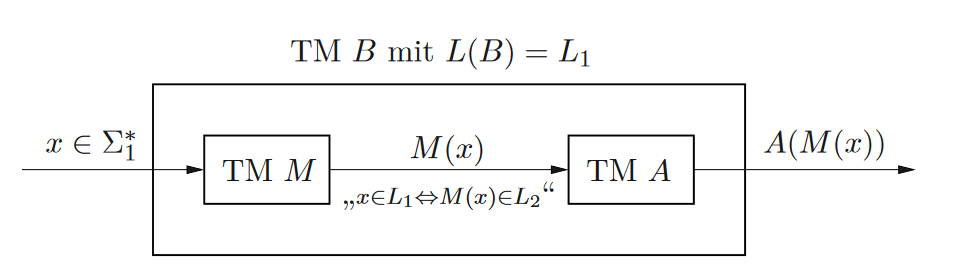
\includegraphics[width=0.8\textwidth]{Images/Basic_EE-Reduktion.png}
                    \caption{Abbildung 5.7 vom Buch}
                \end{figure}
            
            
            
                \subsection{Verhältnis von EE-Reduktion und R-Reduktion}
                \begin{mainbox}{Lemma 5.3}
                    Seien $L_1 \subseteq \Sigma_{1}^*$ und $L_2 \subseteq \Sigma_{2}^*$ zwei Sprachen.
                    $$L_1 \leq_{\text{EE}} L_2 \implies L_1 \leq_{\text{R}} L_2$$
                \end{mainbox}
                \textbf{Beweis: }
                $$L_1 \leq_{\text{EE}} L_2 \implies \exists \text{TM } M. \ x \in L_1 \iff M(x) \in L_2$$
            
                Wir zeigen nun $L_1 \leq_{\text{R}} L_2$, i.e. $L_2 \in \Lr \implies L_1 \in \Lr$.
            
                Sei $L_2 \in \Lr$. Dann existiert ein Algorithmus $A$ (TM, die immer hält), der $L_2$ entscheidet.

                Wir konstruieren eine TM $B$ (die immer hält) mit $L(B) = L_1$
            
                Für eine Eingabe $x \in \Sigma_1^*$ arbeitet $B$ wie folgt:
                \begin{enumerate}[label=(\roman*)]
                    \item $B$ simuliert die Arbeit von $M$ auf $x$, bis auf dem Band das Wort $M(x)$ steht.
                    \item $B$ simuliert die Arbeit von $A$ auf $M(x)$.
                    
                    Wenn $A$ das Wort $M(x)$ akzeptiert, dann akzeptiert $B$ das Wort $x$.
            
                    Wenn $A$ das Wort $M(x)$ verwirft, dann verwirft $B$ das Wort $x$.
                \end{enumerate}
                $A$ hält immer $\implies$ $B$ hält immer und somit gilt $L_1 \in \Lr$  
            
                $\hfill\blacksquare$
            
            
            
                \subsection{$L$ und $L^\complement$}

                \begin{mainbox}{Lemma 5.4}
                    Sei $\Sigma$ ein Alphabet. Für jede Sprache $L \subseteq \Sigma^*$ gilt:
                 $$L \leq_\text{R} L^\complement \text{ und } L^\complement \leq_\text{R} L$$
                \end{mainbox}
                \textbf{Beweis: }
            
                Es reicht $L^\complement \leq_\text{R} L$ zu zeigen, da $(L^\complement)^\complement = L$ und somit dann $(L^\complement)^\complement = L \leq_\text{R} L^\complement$.
            
                Sei $M'$ ein Algorithmus für $L$, der immer hält ($L \in \L_\text{R}$). Dann beschreiben wir einen Algorithmus $B$, der $L^\complement$ entscheidet. 
                
                $B$ übernimmt die Eingaben und gibt sie an $M'$ weiter und invertiert dann die Entscheidung von $M'$. Weil $M'$ immer hält, hält auch $B$ immer und wir haben offensichtlich $L(B) = L$.
            
                \hspace*{0pt}\hfill$\blacksquare$
            
                
                \begin{subbox}{Korollar 5.2}
                    $$(L_\text{diag})^\complement \notin \L_\text{R}$$
                \end{subbox}
                
                \textbf{Beweis:} 
                
                Aus Lemma 5.4 haben wir $L_\text{diag} \leq_\text{R} (L_\text{diag})^\complement$. Daraus folgt $L_\text{diag} \notin \Lr \implies (L_\text{diag})^\complement \notin \Lr$.
                Da $L_\text{diag} \notin \Lre$ gilt auch $L_\text{diag} \notin \Lr$. 
                
                Folglich gilt $(L_\text{diag})^\complement \notin \Lr$.
            
                \hspace*{0pt}\hfill$\blacksquare$
            
            
            
              

                \begin{mainbox}{Lemma 5.5}
                    $$L_{\text{diag}}^{\complement} \in \Lre$$
                \end{mainbox}
                \textbf{Beweis}
                    
                
                    Direkter Beweis: Wir beschreiben eine TM $A$ mit $L(A) = L_{\text{diag}}^\complement$.
                    
                    \textbf{Eingabe}: $x \in (\Sigma_{\text{bool}})^*$
                    
                    \begin{enumerate}[label=(\roman*)]
                        \item Berechne $i$, so dass $w_i = x$ in kanonischer Ordnung
                        \item Generiere $\text{Kod}(M_i)$.
                        \item Simuliere die Berechnung von $M_i$ auf $w_i = x$. 
                    \end{enumerate}
                   
                
                    \begin{itemize}[label=-]
                        \item Falls $w_i \in L(M_i)$ akzeptiert, akzeptiert $A$ die Eingabe $x$.
                        \item Falls $M_i$ verwirft (hält in $q_{\text{reject}}$), dann hält $A$ und verwirft $x = w_i$ auch.
                        \item Falls $M_i$ unendlich lange arbeitet, wird $A$ auch nicht halten und dann folgt auch $x \notin L(A)$.  
                    \end{itemize}
                    Aus dem folgt $L(A) = L_{\text{diag}}^\complement$.
                
                    $\hfill\blacksquare$
                    \begin{subbox}{Korollar 5.3}
                        $L_{\text{diag}}^\complement \in \Lre \setminus \Lr$ und daher $\Lr \subsetneq \Lre$.
                    \end{subbox}
                
                
                
                    \subsection{Universelle Sprache}
                    Sei 
                    $$L_U := \{\text{Kod}(M)\#w \mid w \in (\Sigma_{\text{bool}})^* \text{ und } M \text{ akzeptiert }w\}$$
                    \begin{mainbox}{Satz 5.6}
                        Es gibt eine TM $U$, \textbf{universelle TM} genannt, so dass 
                        $$L(U) = L_U$$
                        Daher gilt $L_U \in \Lre$.
                    \end{mainbox} 
                    \textbf{Beweis}
                
                    Direkter Beweis: Konstruktion einer TM.
                
                    \textit{Siehe Buch/Vorlesung.}
                
                    \begin{mainbox}{Satz 5.7}
                        $$L_U \notin \Lr$$
                    \end{mainbox}
                    \textbf{Beweis}
                
                    Wir zeigen $L_{\text{diag}}^\complement \leq_{\text{R}} L_U$.
                
                    \textit{Siehe Buch/Vorlesung.}
                    \subsection{Halteproblem}
                    Sei $$L_H = \{\text{Kod}(M)\#w \mid M \text{ hält auf }w\}$$
                    \begin{mainbox}{Satz 5.8}
                        $$L_H \notin \Lr$$
                    \end{mainbox}
                    \textbf{Beweis}
                
                    Wir zeigen $L_U \leq_{\text{R}} L_H$.
                
                    \textit{Siehe Buch/Vorlesung.}
                
                
                
                
                
                    \subsection{Parallele Simulation vs Nichtdeterminismus}
                    Sei 
                    $$L_{\text{empty}} = \{\text{Kod}(M) \mid L(M) = \emptyset\}$$
                    und 
                    $$L_{\text{empty}}^\complement = \{\text{Kod}(M) \mid L(M) \neq \emptyset\} \cup \{x \in \{0,1, \#\}\mid x \notin \textbf{KodTM}\}$$
                    \begin{mainbox}{Lemma 5.6}
                        $$L_{\text{empty}}^\complement \in \Lre$$
                    \end{mainbox}
                
                
                
                    \myTitle{Nichtdeterminismus}

                    \textbf{Beweis}
                
                    Da für jede NTM $M_1$ eine TM $M_2$ existiert mit $L(M_1) = L(M_2)$, reicht es eine NTM $M_1$ mit $L(M_1) = L_{\text{empty}}^\complement$ zu finden.
                
                    Eingabe: $x \in \{0,1,\#\}$
                    \begin{enumerate}[label=(\roman*)]
                        \item $M_1$ prüft deterministisch, ob $x = \text{Kod}(M)$ für eine TM $M$. 
                        
                        Falls $x$ keine TM kodiert, wird $x$ akzeptiert.
                        
                        \item Sonst gilt $x = \text{Kod}(M)$ für eine TM $M$ und $M_1$ wählt nichtdeterministisch ein Wort $y \in (\Sigma_{\text{bool}})^*$. 
                        
                        \item Dann simuliert $M_1$ die TM $M$ auf $y$ deterministisch und übernimmt die Ausgabe. 
                    \end{enumerate} 
                
                
                    Wir unterscheiden zwischen 3 Fällen
                    \begin{enumerate}[label = \Roman*]
                        
                        \item $x = \text{Kod}(M)$ und $L(M) = \emptyset$
                        
                        Dann gilt $x \notin L_{\text{empty}}^\complement$ und da es keine akzeptierende Berechnung gibt, auch $x \notin L(M_1)$.
                        
                        \item $x = \text{Kod}(M)$ und $L(M) \neq \emptyset$
                        
                        Dann gilt $x \in L_{\text{empty}}^\complement$ und da es eine akzeptierende Berechnung gibt, auch $x \in L(M_1)$.
                        
                        \item $x$ kodiert keine TM
                        
                        Wir haben $x \in L_{\text{empty}}^\complement$ und wegen Schritt (i) auch $x \in L(M_1)$.
                    \end{enumerate}
                    Somit gilt $L(M_1) = L_{\text{empty}}^\complement$.
                
                    $\hfill\blacksquare$
                
                
                
                    \myTitle{Parallele Simulation}

                    \textbf{Alternativer Beweis}
                
                    Wir konstruieren eine TM $A$ mit $L(A) = L$ direkt.
                    Eingabe: $x \in \{0,1,\#\}$
                    \begin{enumerate}[label=\Roman*.]
                        
                        \item Falls $x$ keine Kodierung einer TM ist, akzeptiert $A$ die Eingabe.
                        
                        \item Falls $x = \text{Kod}(M)$ für eine TM $M$, arbeitet $A$ wie folgt
                        \begin{itemize}[label=-]
                            \item Generiert systematisch alle Paare $(i, j) \in (\N \setminus \{0\}) \times (\N \setminus \{0\})$. (Abzählbarkeit)
                            \item Für jedes Paar $(i, j)$, generiert $A$ das kanonisch $i$-te Wort $w_i$ und simuliert $j$ Berechnungsschritte der TM $M$ auf $w_i$.
                            \item Falls $M$ an ein Wort akzeptiert, akzeptiert $A$ das Wort $x$.
                        \end{itemize}
                    \end{enumerate}
                
                    Falls $L(M) \neq \emptyset$ existiert ein $y \in L(M)$. Dann ist $y = w_k$ für ein $k \in \N\setminus\{0\}$ und die akzeptierende Berechnung von $M$ auf $y$ hat eine endliche Länge $l$.
                
                    Das Paar $(k, l)$ wird in endlich vielen Schritten erreicht und somit akzeptiert $A$ die Eingabe $x$, falls $L(M) \neq \emptyset$.
                
                    Somit folgt $L(A) = L_{\text{diag}}^\complement$.
                
                    $\hfill\blacksquare$
                
                
                
                    \subsection{Aufgabe 5.22}
                    Wir zeigen
                    $$L \in \Lre \land L^\complement \in \Lre \iff L \in \Lr$$
                
                    $\mathbf{(\implies):}$
                    
                    Nehmen wir $L \in \Lre \land L^\complement \in \Lre$ an.
                
                    Dann existiert eine TM $M$ und $M_C$ mit $L(M) = L$ und $L(M_C) = L^\complement$.
                
                    Wir konstruieren eine TM $A$, die für eine Eingabe $w$ die beiden TM's $M$ und $M_C$ parallel auf $w$ simuliert.
                    
                    $A$ akzeptiert $w$, falls $M$ das Wort akzeptiert und verwirft, falls $M_C$ das Wort akzeptiert.
                    
                    Bemerke, dass $L(M) \cap L(M_C) = \emptyset$ und $L(M) \cup L(M_C) = \Sigma^*$.
                
                    Da $w \in L(M)$ oder $w \in L(M_C)$, hält $A$ immer.
                
                    Da $A$ genau dann akzeptiert, falls $w \in L(M)$, folgt $L(A) = L(M) = L$.
                
                    Demnach gilt $L \in \Lr$.
                
                    
                    $\mathbf{(\impliedby):}$
                
                    Nehmen wir $L \in \Lr$ an. Per Lemma 5.4 gilt $L^\complement \leq_{\text{R}} L$ und daraus folgt auch $L^\complement \in \Lr$.
                
                    Da $\Lr \subset \Lre$, folgt $L \in \Lre \land L^\complement \in \Lre$.
                
                    $\hfill\blacksquare$
                
                
                    \begin{mainbox}{Lemma 5.7}
                        $$L_{\text{empty}}^\complement \notin \Lr$$
                    \end{mainbox}
                    \textbf{Beweis }
                
                    Wir zeigen $L_U \leq_{\text{EE}} L_{\text{empty}}^\complement$.
                
                    \textit{Siehe Buch/Vorlesung.}
                   
                
                    \begin{subbox}{Korollar 5.4}
                        $$L_{\text{empty}} \notin \Lr$$
                    \end{subbox}
                    \begin{subbox}{Korollar 5.5}
                        $$L_{\text{EQ}} \notin \Lr$$
                        für $L_{\text{EQ}} = \{\text{Kod}(M)\#\text{Kod}(\overline{M}) \mid L(M) = L(\overline{M})\}$.
                    \end{subbox}
                
                    \subsection{Beispielaufgabe 17a HS22}

                    Beweise $$L_H \leq_{\text{EE}} L_U$$
                    wobei 
                    $$L_H = \{\text{Kod}(M)\#w \mid M\text{ hält auf }w\land w \in (\Sigma_{\text{bool}})^*\}$$
                    und 
                    $$L_U=\{\text{Kod}(M)\#w \mid M \text{ akzeptiert }w \land w \in (\Sigma_{\text{bool}})^*\}$$
                
                
                    \textbf{Lösung}
                
                    Wir wollen $L_H \leq_{\text{EE}} L_U$ zeigen.
                
                        Wir geben die Reduktion zuerst als Zeichnung an.
                
                        \begin{figure}[htp]
                            \centering
                            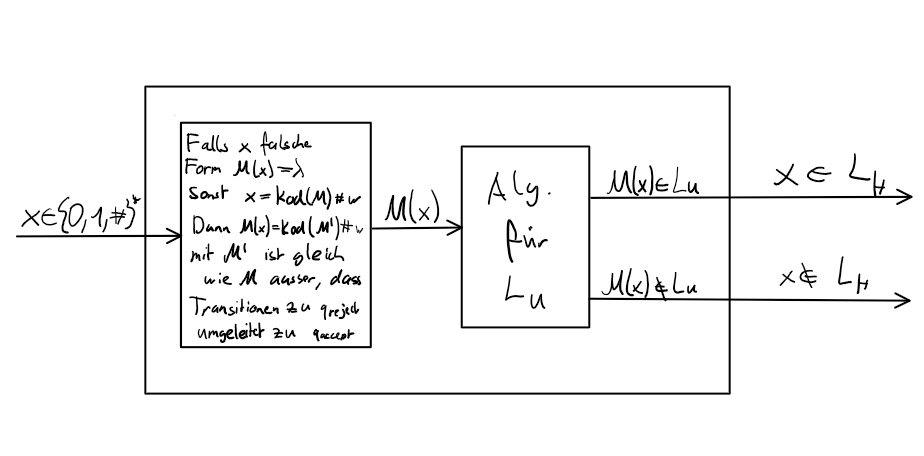
\includegraphics[width = 0.7\textwidth]{Images/17a_Zeichnung.png}
                            \caption{EE-Reduktion von $L_H$ auf $L_U$}
                        \end{figure}
                        
            
                    Wir definieren eine Funktion $M(x)$ für ein $x \in \{0,1,\#\}^*$, so dass
                        $$x \in L_H \iff M(x) \in L_U \qquad (1)$$
                    
                        Falls $x$ nicht die richtige Form hat, ist $M(x) = \lambda$, sonst ist $M(x) = \text{Kod}(M')\#w$ wobei $M'$ gleich aufgebaut ist wie $M$, ausser dass alle Transitionen zu $q_{reject}$ zu $q_{accept}$ umgeleitet werden. Wir sehen, dass $M'$ genau dann $w$ akzeptiert, wenn $M$ auf $w$ hält. 
                        
                        Dieses $M(x)$ übergeben wir dem Algorithmus für $L_U$. 
                
                        
                    Wir beweisen nun $x \in L_H \iff M(x) \in L_U$:
                
                        \begin{enumerate}[label=(\roman*)]
                            \item $x \in L_H$
                
                                Dann ist $x = \text{Kod}(M)\#w$ von der richtigen Form, und $M$ hält auf $w$. 
                                Das heisst die Simulation von $M$ auf $w$ endet entweder in $q_{reject}$ oder in $q_{accept}$. 
                                
                                Folglich wird $M'$ $w$ immer akzeptieren, da alle Transitionen zu $q_{reject}$ zu $q_{accept}$ umgeleitet wurden. 
                                
                                $x \in L_H \implies M(x) \in L_U$
                
                            \item $x \notin L_H$
                
                                Dann unterscheiden wir zwischen zwei Fällen:
                
                                \begin{enumerate}[label=(\alph*)]
                                    \item 
                                    
                                    $x$ hat nicht die richtige Form, i.e. $x \neq \text{Kod}(M)\#w$.
                                    Dann ist $M(x) = \lambda$ und da es keine Kodierung einer Turingmaschine $M$ gibt, so dass Kod$(M) = \lambda$, gilt   $\lambda \notin L_U$.
                            
                
                   
                    \item
                
                                    $x = \text{Kod}(M)\#w$ hat die richtige Form. Dann haben wir $M(x) = $ Kod$(M')\#w$.
                                    
                                    Da aber $x \notin L_H$, hält $M$ nicht auf $w$. Da $M$ nicht auf $w$ hält, erreicht es nie $q_{reject}$ oder $q_{accept}$ in $M$ und so wird $w$ von $M'$ nicht akzeptiert. 
                
                                    $\implies M(x) \notin L_U$
                
                                   
                                    
                                    
                                \end{enumerate}
                                
                                 So haben wir mit diesen Fällen (a) und (b) $x \notin L_H \implies M(x) \notin L_U$ bewiesen. 
                                 
                                 Aus indirekter Implikation folgt $M(x) \in L_U \implies x \in L_H$
                                     
                        \end{enumerate}
                
                   
                
                    Aus (i) und (ii) folgt 
                    
                    $$x \in L_H \iff M(x) \in L_U \qquad (1)$$
                
                    Somit ist die Reduktion korrekt.
                
                    \hspace*{0pt}\hfill$\blacksquare$
                
                
                
                    \subsection{Beispielaufgabe 18b HS22}
    
                    Sei $$L_{\text{infinite}} = \{\text{Kod}(M) \mid \text{$M$ hält auf keiner Eingabe}\}$$
                    Zeige $(L_{\text{infinite}})^C \notin \Lr$
                
                
                    \textbf{Lösung}
    
                    Wir zeigen, dass $(L_{\text{infinite}})^C \notin \Lr$ mit einer geeigneten Reduktion.
                
                    Wir beweisen $L_H \leq_{\text{R}} (L_{\text{infinite}})^C$
                
                    Um dies zu zeigen nehmen wir an, dass wir einen Algorithmus $A$ haben, der $(L_{\text{infinite}})^C$ entscheidet.
                     Wir konstruieren einen Algorithmus $B$, der mit Hilfe von $A$, die Sprache $L_H$ entscheidet. 
                     
                    Wir betrachten folgende Abbildung:
                    
                    \begin{figure}[htp]
                        \centering
                        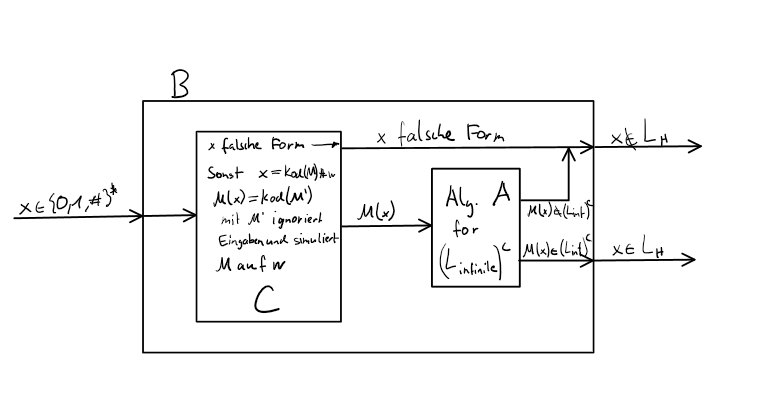
\includegraphics[width=0.75\textwidth]{Images/18b_Zeichnung.png}
                        \caption{R-Reduktion von $L_H$ auf $(L_{\text{infinite}})^C$}
                    \end{figure}
                
                
                    \begin{enumerate}[label=\Roman*.]
                        \item Für eine Eingabe $x \in \{0,1,\#\}^*$ berechnet das Teilprogramm $C$, ob $x$ die richtige Form hat(i.e. ob $x = $ Kod$(M)\#w$ für eine TM $M$).
                        \item Falls nicht, verwirft $B$ die Eingabe $x$.
                        
                        \item Ansonsten, konstruiert $C$ eine Turingmaschine $M'$, die Eingaben ignoriert und immer $M$ auf $w$ simuliert. Wir sehen, dass $M'$ genau dann hält, wenn $M$ auf $w$ hält. 
                        \item Folglich hält $M'$ entweder für jede Eingabe ($M$ hält auf $w$) oder für keine ($M$ hält nicht auf $w$).
                         
                        \item Da $A$ genau dann akzeptiert, wenn die Eingabe keine gültige Kodierung ist(ausgeschlossen, da $C$ das herausfiltert) oder wenn die Eingabe $M(x)= \text{Kod}(M')$ und $M'$ für mindestens eine Eingabe hält, akzeptiert $A$ $M(x)$ genau dann, wenn $x = \text{Kod}(M)\#w$ die richtige Form hat und $M$ auf $w$ hält.
                    \end{enumerate}
                    
                    
                    Folglich gilt $$x \in L_H \iff M(x) \in (L_{\text{infinite}})^C$$
                    $\implies L_H \leq_R (L_{\text{infinite}})^C$ 
                
                    Also folgt die Aussage
                    $$(L_{\text{infinite}})^C \in \L_R \implies L_H \in \L_R$$
                
                    Da wir $L_H \notin \L_R$ (\textbf{Satz 5.8}), folgt per indirekter Implikation:
                    $$(L_{\text{infinite}})^C \notin \L_R$$
                
                    \hspace*{0pt}\hfill$\blacksquare$
                
                \section{Satz von Rice}
                
                
                    \myTitle{Spezialfall des Halteproblems}
                    Wir definieren $L_{\text{H}, \lambda} = \{\text{Kod}(M) \mid M \text{ hält auf }\lambda\}$.
                    \begin{mainbox}{Lemma 5.8}
                        $$L_{\text{H}, \lambda} \notin \Lr$$
                    \end{mainbox}
                    \textbf{Beweis: }
                
                    Wir zeigen $L_\text{H} \leq_\text{EE} L_{\text{H}, \lambda}$. Wir beschreiben einen Algorithmus $B$, so dass $x \in L_\text{H} \iff B(x) \in L_{\text{H}, \lambda}$.
                
                    Für jede Eingabe arbeitet $B$ wie folgt:
                    \begin{itemize}
                        \item Falls $x$ von der falschen Form, dann $B(x) = M_{inf}$, wobei $M_{inf}$ unabhängig von der Eingabe immer unendlich läuft.
                        \item Sonst $x = \text{Kod}(M)\#w$: Dann $B(x) = M'$, wobei $M'$ die Eingabe ignoriert und immer $M$ auf $w$ simuliert.
                    \end{itemize}
                
                    Wir sehen, dass $M'$ genau dann auf $\lambda$ hält, wenn $x \in L_{\text{H}}$.
                
                    Daraus folgt $x \in L_\text{H} \iff B(x) \in L_{\text{H}, \lambda}$.
                
                    \hspace*{0pt}\hfill$\blacksquare$
                
                    \myTitle{Satz von Rice}
                    \begin{mainbox}{Satz 5.9}
                        Jedes semantisch nichttriviale Entscheidungsproblem über Turingmaschinen ist unentscheidbar.
                    \end{mainbox}
                    \begin{itemize}
                        \item 'über Turingmaschinen' = $L \subseteq \textbf{KodTM}$.
                        \item 'nichttrivial' = $\exists M_1: \text{Kod}(M_1) \in L$ und $\exists M_2: \text{Kod}(M_2) \notin L$
                        \item 'semantisch' = Für $A, B$ mit $L(A) = L(B)$ gilt $\text{Kod}(A) \in L \iff \text{Kod}(B) \in L$.
                    \end{itemize}
                
                    
                
                    \subsection{Beispielaufgabe: Satz von Rice}
                    Wir definieren $$L_{\text{all}} = \{\text{Kod}(M) \mid L(M) = (\Sigma_{\text{bool}})^*\}.$$
                
                    Zeige $$L_{\text{all}} \notin \Lr.$$
                
                
                
                
                \section{How To Reduktion}
                
                    \subsection{$L \in \Lr$ }
                        Wir kennen zwei Methoden um dies zu beweisen:
                        \begin{enumerate}[label=\Roman*.]
                            \item \textbf{Reduktion}
                            \begin{enumerate}[label = (\alph*)]
                                \item Wir finden eine Sprache $L' \in \L_\text{R}$ (entweder schon in Vorlesung bewiesen oder selbst beweisen).
                                \item  Zeige die Reduktion $L \leq_{\text{R}} L'$ (folgt trivial aus Lemma 5.4 für $L' = L^\complement$).
                            \end{enumerate}
                                \item \textbf{Direkter Beweis: TM Konstruktion}
                                \begin{enumerate}[label=(\alph*)]
                                    \item Beschreibung einer TM (bzw. ein Algorithmus) $M$ mit $L(M) = L$. Dabei kann man eine schon bekannte TM $A$ verwenden, die immer hält (i.e. $L(A) \in \Lr$).
                                    \item Beweise $L(M) = L$ und dass die TM $M$ \textbf{immer} hält.
                                \end{enumerate}
                        \end{enumerate}
                
                
                
                    \subsection{$L \notin \Lr$}
                        Wir kennen hier auch 3 Arten:
                        \begin{itemize}[label=-]
                            \item \textbf{Trivial}
                            
                            Folgt sofort aus $L \notin \L_{\text{RE}}$, da $\L_{\text{R}} \subset \L_{\text{RE}}$.
                            \item \textbf{Reduktion}
                            \begin{enumerate}[label=(\alph*)]
                               \item Finde eine Sprache $L'$, so dass $L' \notin \L_{\text{R}}$ (muss bewiesen werden, falls nicht im Buch).
                               \item Beweise $L' \leq_{\text{R/EE}} L$.
                               \item Geeignete Sprachen als $L'$ sind: $L_{empty}^\complement, L_{diag}^\complement, L_\text{H}, L_\text{U}, L_{\text{H}, \lambda}$. (Alle im Buch bewiesen)
                            \end{enumerate}
                            \item \textbf{Satz von Rice} 
                        \end{itemize}
                
                
                \subsection{Anwendung von Satz von Rice}
                    Für den \textbf{Satz von Rice}:
                    \begin{itemize}[label=-]
                        \item Wir können mit diesem Satz nur $L \notin \L_{\text{R}}$ beweisen!
                        \item Wir haben folgende Bedingungen:
                        \begin{enumerate}[label=\roman*.]
                            \item $L \subseteq \text{KodTM}$
                            \item $\exists$ TM $M$: Kod$(M) \in L$
                            \item $\exists$ TM $M$: Kod$(M) \notin L$
                            \item $\forall$ TM $M_1, M_2$: $L(M_1) = L(M_2) \implies \left(\text{Kod}(M_1) \in L \iff \text{Kod}(M_2) \in L\right)$
                        \end{enumerate}
                        Für den letzten Punkt (4) muss man überprüfen, ob in der Definition von $L = \{\text{Kod}(M) \mid M \text{ ist TM und ...}\}$ überall nur $L(M)$ vorkommt und nirgends $M$ direkt. 
                        
                        Beziehungsweise reicht es, wenn man die Bedingung so umschreiben kann, dass sie nur noch durch $L(M)$ beschrieben ist.
                    \end{itemize}
                
                
                
                    \subsection{$L \in \L_{\text{RE}}$}
                    \begin{enumerate}[label=\Roman*.]
                        \item  Wir beschreiben eine TM $M$ mit $L(M) = L$, die nicht immer halten muss. 
                        \item  Meistens muss die TM eine Eigenschaft, für alle möglichen Wörter prüfen. 
                        \item  Bsp: $L = \{\text{Kod}(M_1) \mid \text{Kod}(M_1) \in L_\text{H}^\complement\}$: Wir gehen alle Wörter durch, um dasjenige zu finden, für das $M_1$ hält.
                        \item  Wir verwenden oft einen von den folgenden 2 Tricks, um dies zu tun:
                        \begin{itemize}[label=-]
                            \item Da es für jede NTM $M'$, eine TM $M$ gibt, so dass $L(M') = L(M)$, können wir eine solche definieren, für die $L(M') = L$ gilt.
                            \item Die andere Variante, ist die parallele Simulation von Wörtern, bei dem man das Diagonalisierungsverfahren aus dem Buch verwendet. (Bsp: Beweis $L_{\text{empty}} \in \L_{\text{RE}}$, S. 156 Buch)
                        \end{itemize}
                    \end{enumerate}
                
                    \subsection{$L \notin \L_{\text{RE}}$}
                        Hier haben wir 2 mögliche (offizielle) Methoden:
                        \begin{itemize}[label=-]
                            \item Diagonalisierungsargument mit Widerspruch, wie beim Beweis von $L_{\text{diag}} \notin \L_{\text{RE}}$.
                            \item Widerspruchsbeweis mit der Aussage $L \in \L_{\text{RE}} \land L^\complement \in \L_{\text{RE}} \implies L \in \L_{\text{R}}$ (Aufgabe 5.22, muss begründet werden!).
                        \end{itemize}
                        Inoffiziell könnten wir auch die EE-Reduktion verwenden, wird aber weder in der Vorlesung noch im Buch erwähnt.
                    
                
                
                
                    \subsection{EE- und R-Reduktionen: Tipps und Tricks}
                        \begin{itemize}[label=-]
                            \item Die vorgeschaltete TM $A$ muss immer terminieren! I.e. sie muss ein Algorithmus sein.
                            
                            \item Die Eingabe sollte immer zuerst auf die Richtige Form überprüft werden!
                            
                            Auch im Korrektsheitsbeweis, sollte dieser Fall als erstes abgehandelt werden.
                            \item Für Korrektheit müssen wir immer $x \in L_1 \iff A(x) \in L_2$ beweisen.
                            
                            \item Wir verwenden meistens folgende 2 Tricks:
                            \begin{enumerate}[label=\roman*.]
                                \item Transitionen nach $q_{accept}$ oder $ q_{reject}$ umleiten nach $q_{reject}$/$q_{accept}$ oder einer \textbf{Endlosschleife}. 
                                \item TM $M'$ konstruieren, die ihre Eingabe ignoriert und immer dasselbe tut (z.B. eine TM dessen Kodierung gegeben ist, auf ein fixes Wort simuliern).
                            \end{enumerate}
                            
                            \item Die Kodierung einer TM generieren, dessen Sprache gewisse Eigenschaften hat(z.B. sie akzeptiert alle Eingaben, läuft immer unendlich etc.)
                        \end{itemize}
                
            
            % \section{How To Reduktion}
            
            %     \subsection{$L \in \Lr$ }

            %         Wir kennen zwei Methoden um dies zu beweisen:
            %         \begin{itemize}[label=-]
            %             \item Wir finden eine Sprache $L' \in \L_\text{R}$ und zeigen $L \leq_{\text{R}} L'$. (Meistens ein wenig umständlich)
            %             \item Direkter Beweis:  Eine TM (bzw. ein Algorithmus) $A$ beschreiben, so dass $L(A) = L$ und $A$ immer terminiert.
            %         \end{itemize}
            
            
            
            %     \subsection{$L \notin \Lr$}

            %         Wir kennen hier auch 3 Arten:
            %         \begin{itemize}[label=-]
            %             \item Folgt sofort aus $L \notin \L_{\text{RE}}$, da $\L_{\text{R}} \subset \L_{\text{RE}}$.
            %             \item Wir wählen eine Sprache $L'$, so dass $L' \notin \L_{\text{R}}$ und beweisen $L' \leq_{\text{R/EE}} L$.
                        
            %                 Geeignete Sprachen als $L'$ sind: $L_{empty}^\complement, L_{diag}^\complement, L_\text{H}, L_\text{U}, L_{\text{H}, \lambda}$. (Alle im Buch bewiesen)
            %             \item Satz von Rice 
            %         \end{itemize}
            
            
            % \subsection{Anwendung von Satz von Rice}

            %     Für den \textbf{Satz von Rice}:
            %     \begin{itemize}[label=-]
            %         \item Wir können mit diesem Satz nur $L \notin \L_{\text{R}}$ beweisen!
            %         \item Wir haben folgende Bedingungen:
            %         \begin{enumerate}[label=\roman*.]
            %             \item $L \subseteq \text{KodTM}$
            %             \item $\exists$ TM $M$: Kod$(M) \in L$
            %             \item $\exists$ TM $M$: Kod$(M) \notin L$
            %             \item $\forall$ TM $M_1, M_2$: $L(M_1) = L(M_2) \implies \left(\text{Kod}(M_1) \in L \iff \text{Kod}(M_2) \in L\right)$
            %         \end{enumerate}
            %         Für den letzten Punkt (4) muss man überprüfen, ob in der Definition von $L = \{\text{Kod}(M) \mid M \text{ ist TM und ...}\}$ überall nur $L(M)$ vorkommt und nirgends $M$ direkt. Beziehungsweise reicht es, wenn man die Bedingung so umschreiben kann, dass sie nur noch durch $L(M)$ beschrieben ist.
            %     \end{itemize}
            
            
            
            %     \subsection{$L \in \L_{\text{RE}}$}

            %         Wir beschreiben eine TM $M$ mit $L(M) = L$, die nicht immer halten muss. 
                    
            %         Meistens muss die TM eine Eigenschaft, für alle möglichen Wörter prüfen. (Bsp: $\text{Kod}(M_1) \in L_\text{H}^\complement$: Wir gehen alle Wörter durch, um dasjenige zu finden, für das $M_1$ hält.)
                    
            %         Wir verwenden oft einen von den folgenden 2 Tricks, um dies zu tun:
            %         \begin{itemize}
            %             \item Da es für jede NTM $M'$, eine TM $M$ gibt, so dass $L(M') = L(M)$, können wir eine solche definieren, für die $L(M') = L$ gilt.
            %             \item Die andere Variante, ist die parallele Simulation von Wörtern, bei dem man das Diagonalisierungsverfahren aus dem Buch verwendet. (Bsp: Beweis $L_{\text{empty}} \in \L_{\text{RE}}$, S. 156 Buch)
            %         \end{itemize}
            
            
            
            %     \subsection{$L \notin \L_{\text{RE}}$}

            %         Hier haben wir 2 mögliche (offizielle) Methoden:
            %         \begin{itemize}[label=-]
            %             \item Diagonalisierungsargument mit Widerspruch, wie beim Beweis von $L_{\text{diag}} \notin \L_{\text{RE}}$.
            %             \item Widerspruchsbeweis mit der Aussage $L \in \L_{\text{RE}} \land L^\complement \in \L_{\text{RE}} \implies L \in \L_{\text{R}}$.
            %         \end{itemize}
            %         Inoffiziell könnten wir auch die EE-Reduktion verwenden, wird aber weder in der Vorlesung noch im Buch erwähnt.
            
            %     \subsection{EE- und R-Reduktionen: Tipps und Tricks}

            %         \begin{itemize}[label=-]
            %             \item Die vorgeschaltete TM $A$ muss immer terminieren! I.e. sie muss ein Algorithmus sein.
                        
            %             \item Die Eingabe sollte immer zuerst auf die Richtige Form überprüft werden!
                        
            %             Auch im Korrektsheitsbeweis, sollte dieser Fall als erstes abgehandelt werden.
            %             \item Für Korrektheit müssen wir immer $x \in L_1 \iff A(x) \in L_2$ beweisen.
                        
            %             \item Wir verwenden meistens folgende 2 Tricks:
            %             \begin{enumerate}[label=\roman*.]
            %                 \item Transitionen nach $q_{accept}$ oder $ q_{reject}$ umleiten nach $q_{reject}$/$q_{accept}$ oder einer \textbf{Endlosschleife}. 
            %                 \item TM $M'$ konstruieren, die ihre Eingabe ignoriert und immer dasselbe tut (z.B. eine TM dessen Kodierung gegeben ist, auf ein fixes Wort simuliern).
            %             \end{enumerate}
                        
            %             \item Die Kodierung einer TM generieren, dessen Sprache gewisse Eigenschaften hat(z.B. sie akzeptiert alle Eingaben, läuft immer unendlich etc.)
            %         \end{itemize}
    




    % --------------------------------------------------------------------------------------------
    % Beweise

%     \section{Beweisesammlung}

%     \subsubsection*{Lemma 5.4}
%     Sei $\Sigma$ ein Alphabet. Für jede Sprache $L \subseteq \Sigma^*$ gilt:
    
%     $$L \leq_\text{R} L^\complement \text{ und } L^\complement \leq_\text{R} L$$

%     \textbf{Beweis: }
%     Es reicht $L^\complement \leq_\text{R} L$ zu zeigen, da $(L^\complement)^\complement = L$ und somit dann $(L^\complement)^\complement = L \leq_\text{R} L^\complement$.

%     Sei $M'$ ein Algorithmus für $L$, der immer hält ($L \in \L_\text{R}$). Dann beschreiben wir einen Algorithmus $B$, der $L^\complement$ entscheidet. 
    
%     $B$ übernimmt die Eingaben und gibt sie an $M'$ weiter und invertiert dann die Entscheidung von $M'$. Weil $M'$ immer hält, hält auch $B$ immer und wir haben offensichtlich $L(B) = L$.

%     \hspace*{0pt}\hfill$\blacksquare$

%     \subsubsection*{Korollar 5.2 (bzw. Anwendung von Lemma 5.4)}
%     $(L_\text{diag})^\complement \notin \L_\text{R}$.
    
%     \textbf{Beweis:} 
    
%     Aus Lemma 5.4 haben wir $L_\text{diag} \leq_\text{R} (L_\text{diag})^\complement$. Daraus folgt $L_\text{diag} \notin \Lr \implies (L_\text{diag})^\complement \notin \Lr$.
%     Da $L_\text{diag} \notin \Lre$ gilt auch $L_\text{diag} \notin \Lr$. 
    
%     Folglich gilt $(L_\text{diag})^\complement \notin \Lr$.

%     \hspace*{0pt}\hfill$\blacksquare$

    
   
%     \subsubsection*{Lemma 5.8}
%     $L_{\text{H}, \lambda} \notin \Lr$.

%     \textbf{Beweis: }

%     Wir zeigen $L_\text{H} \leq_\text{EE} L_{\text{H}, \lambda}$. Wir beschreiben einen Algorithmus $B$, so dass $x \in L_\text{H} \iff B(x) \in L_{\text{H}, \lambda}$.

%     Für jede Eingabe arbeitet $B$ wie folgt:
%     \begin{itemize}
%         \item Falls $x$ von der falschen Form, dann $B(x) = M_{inf}$, wobei $M_{inf}$ unabhängig von der Eingabe immer unendlich läuft.
%         \item Sonst $x = \text{Kod}(M)\#w$: Dann $B(x) = M'$, wobei $M'$ die Eingabe ignoriert und immer $M$ auf $w$ simuliert.
%     \end{itemize}

%     Wir sehen, dass $M'$ genau dann auf $\lambda$ hält, wenn $x \in L_{\text{H}}$.

%     Daraus folgt $x \in L_\text{H} \iff B(x) \in L_{\text{H}, \lambda}$.

%     \hspace*{0pt}\hfill$\blacksquare$

%     \subsection*{Kapitel 6}
    
%     \subsubsection*{Lemma 6.1}
%     Sei $k$ eine positive ganze Zahl. Für jede $k$-Band Turingmaschine $A$, die immer hält, existiert eine äquivalente $1$-Band-TM $B$, so dass
%     $$\text{Space}_B(n) \leq \text{Space}_A(n)$$

%     \textbf{Beweisskizze: }

%     Gleiche Konstruktion wie in Lemma 4.2. Wir können leicht sehen, dass $B$ genau so viele Felder braucht, wie $A$.


%     \subsubsection*{Lemma 6.2}
%     Zu jeder MTM $A$ existiert eine äquivalente MTM $B$ mit 
%     $$\text{Space}_B(n) \leq \frac{\text{Space}_A(n)}{2}+2$$

%     \textbf{Beweisskizze: }

%     Wir fassen jeweils 2 Felder von $A$ zu einem Feld in $B$ zusammen. $\Gamma_B = \Gamma_A \times \Gamma_A$. Wir addieren $1$ für das $\cent$ am linken Rand und $1$ für das Aufrunden im Fall von ungerader Länge.

%     \subsubsection*{Lemma 6.3}
%     TIME($t$) $\subseteq$ SPACE($t$)

%     \textbf{Beweisskizze: }
%     In $t$ Schritten sind höchstens $t$ Felder beschreibbar.

%     \subsubsection*{Lemma 6.4}
%     Sei $S$ platzkonstruierbar. Für jede MTM $M$, für welche Space$_M(w) \leq s(|w|)$ nur für alle $w \in L(M)$ erfüllt, existiert eine äquivalente MTM $M'$, welche dies für alle $w \in \Sigma^*$ erfüllt.

%     \textbf{Beweisskizze: }
%     Erzeuge für jede Eingabe $x \in \Sigma^*$ zuerst $0^{s(|x|)}$ auf einem zusätzlichen Band und nutze das als Platzüberwachung. Wenn $M'$ diesen Platz überschreiten will, wird die Simulation unterbrochen und die Eingabe verworfen.

%     \subsubsection*{Lemma 6.5}
%     Sei $t$ zeitkonstruierbar. Zu jeder MTM, welche Time$_M(w) \leq t(|w|)$ nur für alle $w \in L(M)$ erfüllt, existiert eine äquivalente MTM $M'$, welche zumindest Time$_M(w) \leq 2t(|w|) \in \O(t(|w|))$ für alle $w \in \Sigma^*$ erfüllt.

%     \textbf{Beweisskizze: }
%     Schreibe für jede Eingabe $x \in \Sigma^*$ $0^{t(|x|)}$ auf ein zusätzliches Arbeitsband und nutze dies zur Zeitzählung. Wenn $M'$ mehr Schritte machen will, wird die Simulation abgebrochen und die Eingabe verworfen.

%     \subsubsection*{Satz 6.2}
%     Für jede Funktion $s$ mit $s(n) \geq \log_2(n)$ gilt:

%     $$\textbf{SPACE}(s(n)) \subseteq \bigcup_{c \in \N} \textbf{TIME}(c^{s(n)})$$

%     \textbf{Beweis: } 

%     Sei $L \in \textbf{SPACE}(s(n))$. Nach Lemma 6.1 existiert eine 1-Band-TM $M=(Q,\Sigma,\Gamma,\delta,q_0,q_{accept},q_{reject})$, die \textbf{immer hält}, so dass $L = L(M)$ und Space$_M(n) \leq d \cdot s(n)$ für $d \in \N$ gelten. Für jede Konfiguration $C =(q,w,i,x,j)$ von $M$ definieren wir die \textbf{innere Konfiguration von $C$} als $$\text{In}(C) = (q,i,x,j).$$ 
%     Die innere Konfiguration enthält das Eingabewort $w$ nicht, da dies sich während einer Berechnung nicht ändert. 

%     Wir betrachten die Menge aller inneren Konfigurationen , dass bei einer \textbf{deterministischen} TM jede Berechnung $D = C_1,C_2,C_3, ...$ von $M$ auf einem Wort $w$ mit $|w| = n$, die länger als 





% %-----------------------------------------------------------------



% %------------------------------------------------------------------

%     \section{EE-Reduktionen und R-Reduktionen -- Komplexitätsbeweise}
%     \textit{Mit Inspiration von der Zsf. von Fabian Frei}

%     Generelle Bemerkungen:
%     \begin{itemize}
%         \item $L$ rekursiv (entscheidbar) $\iff$ $L \in \L_{\text{R}}$
%         \item $L$ rekursiv aufzählbar $\iff$ $L \in \L_{\text{RE}}$
%         \item "Algorithmus" ist ein anderes Wort für eine Turingmaschine, die \textbf{immer} terminiert.
%     \end{itemize}
%     \subsection{$L \in \L_\text{R}$ }
%     Wir kennen zwei Methoden um dies zu beweisen:
%     \begin{itemize}
%         \item Wir finden eine Sprache $L' \in \L_\text{R}$ und zeigen $L \leq_{\text{R}} L'$. (Meistens ein wenig umständlich)
%         \item Direkter Beweis:  Eine TM (bzw. ein Algorithmus) $A$ beschreiben, so dass $L(A) = L$ und $A$ immer terminiert.
%     \end{itemize}
%     \subsection{$L \notin \L_{\text{R}}$}
%     Wir kennen hier auch 3 Arten:
%     \begin{itemize}
%         \item Folgt sofort aus $L \notin \L_{\text{RE}}$, da $\L_{\text{R}} \subset \L_{\text{RE}}$.
%         \item Wir wählen eine Sprache $L'$, so dass $L' \notin \L_{\text{R}}$ und beweisen $L' \leq_{\text{R/EE}} L$.
        
%             Geeignete Sprachen als $L'$ sind: $L_{empty}^\complement, L_{diag}^\complement, L_\text{H}, L_\text{U}, L_{\text{H}, \lambda}$. (Alle im Buch bewiesen)
%         \item Satz von Rice 
%     \end{itemize}

%     Für den \textbf{Satz von Rice}:
%     \begin{itemize}
%         \item Wir können mit diesem Satz nur $L \notin \L_{\text{R}}$ beweisen!
%         \item Wir haben folgende Bedingungen:
%         \begin{enumerate}
%             \item $L \subseteq \text{KodTM}$
%             \item $\exists$ TM $M$: Kod$(M) \in L$
%             \item $\exists$ TM $M$: Kod$(M) \notin L$
%             \item $\forall$ TM $M_1, M_2$: $L(M_1) = L(M_2) \implies \left(\text{Kod}(M_1) \in L \iff \text{Kod}(M_2) \in L\right)$
%         \end{enumerate}
%         Für den letzten Punkt (4) muss man überprüfen, ob in der Definition von $L = \{\text{Kod}(M) \mid M \text{ ist TM und ...}\}$ überall nur $L(M)$ vorkommt und nirgends $M$ direkt. Beziehungsweise reicht es, wenn man die Bedingung so umschreiben kann, dass sie nur noch durch $L(M)$ beschrieben ist.
%     \end{itemize}
    
    
%     \subsection{$L \in \L_{\text{RE}}$}
%     Wir beschreiben eine TM $M$ mit $L(M) = L$, die nicht immer halten muss. 
    
%     Meistens muss die TM eine Eigenschaft, für alle möglichen Wörter prüfen. (Bsp: $\text{Kod}(M_1) \in L_\text{H}^\complement$: Wir gehen alle Wörter durch, um dasjenige zu finden, für das $M_1$ hält.)
    
%     Wir verwenden oft einen von den folgenden 2 Tricks, um dies zu tun:
%     \begin{itemize}
%         \item Da es für jede NTM $M'$, eine TM $M$ gibt, so dass $L(M') = L(M)$, können wir eine solche definieren, für die $L(M') = L$ gilt.
%         \item Die andere Variante, ist die parallele Simulation von Wörtern, bei dem man das Diagonalisierungsverfahren aus dem Buch verwendet. (Bsp: Beweis $L_{\text{empty}} \in \L_{\text{RE}}$, S. 156 Buch)
%     \end{itemize}

%     \subsection{$L \notin \L_{\text{RE}}$}
%     Hier haben wir 2 mögliche (offizielle) Methoden:
%     \begin{itemize}
%         \item Diagonalisierungsargument mit Widerspruch, wie beim Beweis von $L_{\text{diag}} \notin \L_{\text{RE}}$.
%         \item Widerspruchsbeweis mit der Aussage $L \in \L_{\text{RE}} \land L^\complement \in \L_{\text{RE}} \implies L \in \L_{\text{R}}$.
%     \end{itemize}
%     Inoffiziell könnten wir auch die EE-Reduktion verwenden, wird aber weder in der Vorlesung noch im Buch erwähnt.

%     \subsection{EE- und R-Reduktionen: Tipps und Tricks}
%     \begin{itemize}
%         \item Die vorgeschaltete TM $A$ muss immer terminieren! I.e. sie muss ein Algorithmus sein.
%         \item Die Eingabe sollte immer zuerst auf die Richtige Form überprüft werden!
        
%         Auch im Korrektsheitsbeweis, sollte dieser Fall als erstes abgehandelt werden.
%         \item Für Korrektheit müssen wir immer $x \in L_1 \iff A(x) \in L_2$ beweisen.
%         \item Wir verwenden meistens folgende 2 Tricks:
%         \begin{enumerate}
%             \item Transitionen nach $q_{accept}$ oder $ q_{reject}$ umleiten nach $q_{reject}$/$q_{accept}$ oder einer \textbf{Endlosschleife}. 
%             \item TM $M'$ konstruieren, die ihre Eingabe ignoriert und immer dasselbe tut (z.B. eine TM dessen Kodierung gegeben ist, auf ein fixes Wort simuliern).
%         \end{enumerate}
%         \item Die Kodierung einer TM generieren, dessen Sprache gewisse Eigenschaften hat(z.B. sie akzeptiert alle Eingaben, läuft immer unendlich etc.)
%     \end{itemize}

    



%     \section{Polynomialzeitreduktionen}

%     Typische Aufgabe: $L$ ist NP-Vollständig. Dann müssen wir (i) $L$ in NP und (ii) $L$ ist NP-schwer zeigen.

%     \begin{enumerate}[label = (\roman*)]
%         \item Wir beschreiben eine NTM $M$, so dass $L(M) = L$. $M$ errät (nichtdeterministisch) ein Zertifikat und verfiziert dies (deterministisch) in Polynomialzeit.
%         $M$ akzeptiert, wenn die Verfikation erfolgreich ist.

%         $M$ akzeptiert $\iff$ $M$ hat eine akzeptierende Berechnung
%         \item \begin{itemize}
%              \item Wir nehmen eine Sprache $L'$ die NP-Schwer ist und zeigen $L' \leq_{p} L$.
             
%                 \textbf{Beweisidee: }
                
%                 Wir zeigen eine Reduktion indem wir einen Polynomialzeit Algorithmus $A$ beschreiben, so dass $x \in L \iff A(x) \in L'$.
%                 Wir müssen also folgende 2 Punkte für $A$ beweisen:
%                 \begin{itemize}
%                     \item $x \in L \iff A(x) \in L'$ (meist recht komplex, beide Richtungen einzeln beweisen)
%                     \item $A$ läuft in Polynomialzeit (meist trivial, es reicht eine High-Level Begründung zu geben)
%                 \end{itemize}


%              \item Wir könnten es auch direkt beweisen(wie Beweis vom Satz von Cook). Dies ist aber meist zu komplex.
%         \end{itemize}
%     \end{enumerate}

    




%     \section{Grammatiken}



%     \textbf{Beispiel 10.6}

%     Sei $L = \{a^nb^nc^n \mid n \in \N\}$
   
%     Beweis durch Widerspruch:

%     Sei $L$ kontextfrei. Dann gilt das Pumping Lemma für kontextfreie Sprachen.

%     Sei $n_L$  die Konstante aus dem Pumping Lemma.

%     Dann wählen wir $z = a^{n_L}b^{n_L}c^{n_L}, |z| \geq n_L, z \in L$.

%     Dann gilt für jede Partition $z = uvwxy$ mit (i) $|vx| \geq 1$ und (ii) $|vwx| \leq n_L$, auch (iii) $\{uv^iwx^iy \mid i \in \N\}$.
\end{document}
